%Przykładowy plik ułatwiający złożenie projektu dyplomowego inżynierskiego.
%UWAGA: Generowany napis na stronie tytułowej o treści PROJEKT DYPLOMOWY INŻYNIERSKI został zaproponowany przeze mnie i nie jest, póki co, potwierdzony przez władze wydziału. Przed ostatecznym oddaniem tak złożonej pracy należy upewnić się jaka powinna być treść tego napisu. W momencie gdy uzyskam informację na temat treści tego napisu, dokonam niezbędnych zmian w źródłach.

\documentclass[eng,printmode]{mgr}
%opcje klasy dokumentu mgr.cls zostały opisane w dołączonej instrukcji

%poniżej deklaracje użycia pakietów, usunąć to co jest niepotrzebne
%\usepackage{polski} %przydatne podczas składania dokumentów w j. polskim
\usepackage{polski}
\usepackage[utf8]{inputenc}
\usepackage[T1]{fontenc} %poprawne składanie polskich czcionek
%pakiety do grafiki
\usepackage{graphicx}
\usepackage{subcaption}
\usepackage{psfrag}

%pakiety dodające dużo dodatkowych poleceń matematycznych
\usepackage{amsmath}
\usepackage{amsfonts}

%pakiety wspomagające i poprawiające składanie tabel
\usepackage{supertabular}
\usepackage{array}
\usepackage{tabularx}
\usepackage{hhline}
\usepackage{multirow}
\usepackage{indentfirst}
\usepackage{enumitem}

\usepackage{breqn}

\newcommand{\floor}[1]{\left\lfloor #1 \right\rfloor}
\usepackage[justification=centering]{caption}

%pakiet wypisujący na marginesie etykiety równań i rysunków zdefiniowanych przez \label{}, chcąc wygenerować finalną wersję dokumentu wystarczy usunąć poniższą linię
%\usepackage{showlabels}


%definicje własnych poleceń
\newcommand{\R}{I\!\!R} %symbol liczb rzeczywistych, działa tylko w trybie matematycznym
\newtheorem{theorem}{Twierdzenie}[section] %nowe otoczenie do składania twierdzeń

%dane do złożenia strony tytułowej
\title{System lokalizacji samolotów z wykorzystaniem ADS-B}
\engtitle{Airplane tracking system using ADS-B}
\author{Karol Szpila}
\supervisor{\vfil dr in\.z. Krzysztof Halawa\\
\\ Katedra Informatyki Technicznej}
%\guardian{dr hab. inż. Imię Nazwisko Prof. PWr, I-6} %nie używać jeśli opiekun jest tą samą osobą co prowadzący pracę

%\date{2008} %standardowo u dołu strony tytułowej umieszczany jest bieżący rok, to polecenie pozwala wstawić dowolny rok

%poniżej jest lista kierunków i specjalności na wydziale elektroniki, należy wybrać właściwe lub dopisać jeśli nie ma odpowiednich
\field{Automatyka i Robotyka (AIR)}
\specialisation{Technologie Informacyjne\\ w Systemach Automatyki (ART)}
%\specialisation{Robotyka (ARR)}
%\specialisation{Komputerowe sieci sterowania (ARK)}
%\specialisation{Systemy informatyczne w automatyce (ASI)}
%\specialisation{Komputerowe systemy zarządzania \\procesami produkcyjnymi (ARS)}
%\field{Elektronika i telekomunikacja (EIT)}
%\specialisation{Akustyka (ETA)}
%\specialisation{Aparatura elektroniczna (EAE)}
%\specialisation{Elektroniczne i komputerowe \\systemy automatyki (ESA)}
%\specialisation{Zastosowania inżynierii komputerowej \\w technice (EZI)}
%\specialisation{Inżynieria dźwięku (EID)}
%\specialisation{Elektronika stosowana \\i optokomunikacja (TEO)}
%\specialisation{Telekomunikacyjne sieci szerokopasmowe (TSS)}
%\specialisation{Teleinformatyczne sieci mobilne (TSM)}
%\specialisation{Sygnały w telekomunikacji cyfrowej (TSC)}
%\specialisation{Teleinformatyczne systemy rozsiewcze (TSR)}
%\field{Informatyka (INF)}
%\specialisation{Systemy informatyki w medycynie \\i technice (IMT)}
%\specialisation{Inżynieria systemów informatycznych (INS)}
%\specialisation{Inżynieria internetowa (INT)}
%\specialisation{Systemy i sieci komputerowe (ISK)}
%\field{Teleinformatyka (TIN)}
%\specialisation{Teleinformatyka (TIN)}

%tutaj zaczyna się właściwa treść dokumentu
\begin{document}
%\bibliographystyle{plabbrv} %tylko gdy używamy BibTeXa, ustawia polski styl bibliografii

\maketitle %polecenie generujące stronę tytułową
%\dedication{6cm}{To jest przykładowa treść opcjonalnej dedykacji, należy ją zmienić lub usunąć w całości polecenie \texttt{$\backslash$dedication}}

\tableofcontents %spis treści

%poniżej znajduje się przykładowa treść dalszej części dokumentu, zainteresowanych zachęcam do rozszyfrowania frazy "Lorem ipsum" :)
\let\cleardoublepage\clearpage %usuwa puste strony pomiaedzy rozdziałami

\chapter{ Wstęp }
ADS-B (ang. Automatic Dependent Surveillance–Broadcast) to system służący do śledzenia statków powietrznych wykorzystywany w kontroli ruchu powietrznego. Powstał, aby uzupełniać pracę PSR (ang. Primary Surveilance Radar) i w przyszłości całkowicie go zastąpić. PSR jest radarem aktywnym bazującym na wysyłaniu fal elektromagnetycznych oraz pomiarze czasu ich powrotu po odbiciu od przeszkody. Jako wady takich systemów zaliczamy: brak informacji o wykrytym obiekcie poza jego położeniem i rozmiarem oraz wrażliwość na ukształtowanie terenu i warunki pogodowe. ADS-B bazuje na lokalizacji przy pomocy satelitów GPS. Statki powietrzne w sposób ciągły ustalają własną pozycję oraz nadają drogą radiową swoje położenie, prędkość oraz identyfikator.
\\


SSR (ang. Secondary Surveillance Radar) został stworzony, aby uzupełniać pracę PSR o dodatkowe informacje odebrane od samolotu. Mode-S należy do takich systemów. Zapytania są wysyłane przez ATM (ang. Air Traffic Management) na częstotliwości 1030MHz, natomiast odpowiedzi zajmują pasmo 1090MHz. Nadawcę można zidentyfikować na podstawie 24-bitowego adresu ICAO (ang. International Civil Aviation Organization). ADS-B wykorzystuje Mode-S jako technologię transmisji danych.
 
\begin{table}[ph]
\caption{\textit{ Rodzaje wiadomości Mode-S}}
\label{tab:adsb}
  \centering
  \def\arraystretch{1.3}% 
  \begin{tabular}{|c|c|c|}
  \hline
  \multicolumn{1}{|c|}{Rodzaj wiadomości} & \multicolumn{1}{c|}{Downlink Format} & \multicolumn{1}{c|}{Zawartość} \\\cline{1-3}
  \multirow{4}{*}{Mode-S (56 bitów)} 
  				 & \multicolumn{1}{c|}{DF0} & \multicolumn{1}{c|}{Odpowiedz Short Air to Air ACAS} \\\cline{2-3}
                 & \multicolumn{1}{c|}{DF4} & \multicolumn{1}{c|}{Poziom lotu} \\\cline{2-3}
                 & \multicolumn{1}{c|}{DF5} & \multicolumn{1}{c|}{Identyfikator (Roll-call)} \\\cline{2-3}
                 & \multicolumn{1}{c|}{DF11} & \multicolumn{1}{c|}{Odpowiedz (All-call)} \\\hline
  \multirow{6}{*}{Mode-S (112 bitów)} 
  				 & \multicolumn{1}{c|}{DF16} & \multicolumn{1}{c|}{Odpowiedz Long Air to Air ACAS} \\\cline{2-3}
                 & \multirow{5}{*}{DF17 (ADS-B)} & Pozycja powietrzna \\\hhline{~~~} 
                 &                       & Pozycja lądowa \\\hhline{~~~} 
                 &                       & Status \\\hhline{~~~} 
                 &                       & ID i rodzaj samolotu  \\\hhline{~~~} 
                 &                       & Prędkość powietrzna \\\hline
 \multirow{2}{*}{Mode-S EHS (112 bitów)} 
	& \multicolumn{1}{c|}{DF20} & \multicolumn{1}{c|}{Poziom lotu oraz (BDS 4.0/5.0/6.0)} \\\cline{2-3}
	& \multicolumn{1}{c|}{DF21} & \multicolumn{1}{c|}{ID oraz (BDS 4.0/5.0/6.0)} \\\hline
 \end{tabular}
\end{table}
\newpage

Tabela \ref{tab:adsb} prezentuje podział wiadomości Mode-S ze względu na rozmiar bloku danych oraz DF (ang. Downlink Format), czyli formatu odebranej ramki. Rozróżniamy pakiety krótkie o długości 56 bitów i rozszerzone 112 bitowe. DF0 i DF16 stosuje się w ACAS (ang. Airborne Collision Avoidance System), który służy zapobieganiu kolizji w kontroli ruchu powietrznego. Odpowiedz Short Air to Air (DF0), odbierają stacje ATM, natomiast Long Air to Air (DF16), informują poszczególne statki o możliwości zderzenia. Uczestnicy ruchu wysyłający ramkę DF5 potwierdzają, wyposażenie w transponder Mode-S. Ponadto, wyróżniamy odpowiedzi Mode-S EHS (ang. Enhanced Surveillance) DF20 i DF21 zawierające dodatkowe informacje niedostępne w ADS-B.
Format pakietu zależy od wysłanego przez kontrolę naziemną BDS (ang. Comm-B Data Selector).
Tylko SSR, który wysłał zapytanie Mode-S EHS jest wstanie zdekodować otrzymaną wiadomość, ponieważ nie zawiera ona wysłanego BDS. Poniżej przedstawiono parametry odpowiadające poszczególnym BDS.

\begin{figure}[ph]
  \centering
  \includegraphics[width=\textwidth]{images/bds.png}
  \caption{\textit{ BDS dla wiadomości DF20 i DF21 \\http://www.eurocontrol.int/articles/mode-s-operational-overview}}
\end{figure}

Wiadomość Mode-S można odbierać przy pomocy dowolnego odbiornika dostrojonego na częstotliwość 1090MHz. Tunery z układem RTL2832U da się łatwo przekształcić w SDR (ang. Software Defined Radio).  SDR to system komunikacji radiowej w którym parametry radia są konfigurowane poprzez pogram bez ingerencji w sprzęt. Wspomniane urządzenie jest znacznie tańsze od profesjonalnych rozwiązań, co spopularyzowało ADS-B w zastosowaniach amatorskich. 



\chapter{ Cele i założenia projektowe }
Celem niniejszej pracy było stworzenie prototypu systemu pozwalającego na lokalizację oraz zbieranie danych o statkach powietrznych wyposażonych w transpondery ADS-B. W systemie można wyróżnić dwie zasadnicze części.
Wewnętrzną odpowiedzialna za wykrywanie, zbieranie i dekodowanie wiadomości oraz wizualną, zajmującą się prezentacją danych oraz interakcją z użytkownikiem. Urządzenie jest alternatywą dla drogich i profesjonalny systemów w przypadku zastosowań amatorskich.

\section{Środowisko sprzętowe i wykorzystane narzędzia}
W tym podrozdziale przedstawiono wykorzystanie w systemie urządzenia oraz środowisko programistyczne.
\\


Jako odbiornik radiowy zostanie wykorzystany tuner DVB-T z układem RTL2832U wyposażony w interfejs USB. Urządzenie da się łatwo zamienić w SDR. Zdecydowano się na wykorzystanie mikrokontrolera firmy ST z serii STM32F767, ze względu na posiadanie peryferiów niezbędnych do obsługi urządzeń w systemie oraz dostępność narzędzi i oprogramowania. W projekcie wykorzystano wyświetlacz LCD-TFT o przekątnej 10.1 cala.
Wybrano języki programowania C99 oraz C++11.
Poniżej wymieniono użyte biblioteki:
\begin{itemize}
  \item librtlsdr - obsługa Tunera DVB-T jako SDR,
  \item STM32 USB Host Library - komunikacja mikrokontrolera z radiem poprzez interfejs USB,
  \item STemWin - sterowanie wyświetlaczem z panelem dotykowym,
  \item STM32F7 HAL - konfiguracja mikrokontrolera i obsługa peryferiów.
\end{itemize}


System operacyj FreeRTOS zastosowano w celu zapewnienia wielozadaniowości oraz mechanizmów zarządzania zasobami sprzętowymi. Do programowania urządzenia skorzystano z programator ST-Link z zestawu uruchomieniowego STM32F429I-DISC1. Poniżej zaprezentowano wykorzystane programy:

\begin{itemize}
  \item Atollic True Studio - środowisko do programowania mikrokontrolerów,
  \item STM32CubeMx - generowania kodu konfiguracyjnego dla układów STM32,
  \item CircuitMaker - wykonanie projektu PCB.
\end{itemize}

\chapter{ Architektura sprzętowa}
W tym rozdziale zostanie opisana część sprzętowa projektu. Przedstawiono schemat oraz wykonanie PCB wraz z wykorzystanymi elementami oraz zewnętrznymi urządzeniami.


\section{ Schemat Urządzenia}
\subsection*{Zasilanie}
System jest zasilany z zewnętrznego źródła 5V poprzez port USB typu mini A. Pozwala to na podłączenie PCB do sieci poprzez przetwornicę, akumulatora lub innego urządzenia USB typu Host.  
Stabilizator LM1117 został zastosowany, aby obniżyć napięcie do wartości 3,3V przy jakiej pracują układy scalone znajdujące się na PCB. Kondensatory C5, C6, C7 i C8 zajmują się filtracją zasilania 3,3V i i 5V \cite{regulator}. Rysunek (\ref{fig:pwerPcb}) przedstawia podłączenie poszczególnych elementów.
\vskip 0.5cm
\begin{figure}[!h]
    \centering
    \includegraphics[width=\textwidth]{schematics/power.png}
    \caption{\textit{Schemat części zasilania PCB}}
    \label{fig:pwerPcb}
\end{figure}
\subsection*{Mikrokontroler}
Wykorzystany mikrokontroler to STM32F767ZIT6. Układ został wybrany, ponieważ posiada najmniejszą obudowę (LQFP144) zawierającą wszystkie wymagane peryferia takie jak: LTDC do sterowania wyświetlaczem LCD, kontroler zewnętrznej pamięci pozwalający obsłużyć SDRAM i interfejsy komunikacyjne USB, I2C oraz UART. Poniżej przedstawiono schemat podłączenia  \cite{stmsheet}.

\begin{figure}[!h]
    \centering
    \includegraphics[height=\textwidth, angle=90]{schematics/uC.png}
    \caption{\textit{Schemat podłączenia mikrokontrolera STM32F767ZIT6}}
\end{figure}

\subsection*{Interfejsy komunikacyjne}
System posiada gniazdo na kartę Micro SD, która może zostać wykorzysta, aby przechowywać  skompresowane obrazy dla tła wyświetlacza lub mapy. Do programowania mikrokontrolera wykorzystano interfejs SWD ST-Link. Komunikacja z SDR odbywa się poprzez interfejs USB2.0 Full-Speed wyprowadzony poprzez gniazdo Micro USB-B, pozwalając w ten sposób zaoszczędzić na rozmiarze PCB. System jako Host będzie zasilać podłączony tuner. Zgodnie ze standardem maksymalny prąd wyjściowy wynosi 500mA \cite{usbSpec}. Z tego powodu zastosowano przełącznik STMPS2141STR \cite{usbPower}. W przypadku podania stanu wysokiego na pin USB PSO układ zostanie włączony. Jeżeli nie występują żadne sytuacje nieporządne takie jak przeciążenie prądowe czy zwarcie, zapali się zielona dioda sygnalizująca poprawnie działanie. W przypadku jakichkolwiek problemów prąd zostanie natychmiast odcięty, a układ wystawi stan wysoki na pin FAULT informując o tym mikrokontroler i zapalając czerwoną diodę. W celu zabezpieczania interfejsu przed niepożądanymi wyładowaniami elektrostatycznymi zastosowano układ STMECMF02-4CMX8 dedykowany dla USB2.0, służący do ochrony ESD (ang . Electrostatic Discharge ) , który pełni również funkcję filtru EMI, (ang. Electromagnetic Interference) \cite{emi}. Dalej pokazano schemat połączenia elementów.

\begin{figure}[!h]
    \centering
    \includegraphics[width=\textwidth]{schematics/conn.png}
    \caption{\textit{Schemat połączenia zewnętrznych interfejsów}}
\end{figure}

\subsection*{Wyświetlacz}
Zgodnie z założeniem, system ma posiadać interfejs  użytkownika. Do tego celu wybrano wyświetlacz HY101CTP o przekątnej 10,1" i rozdzielczości 1024 na 600 pikseli. Matryca jest sterowana poprzez MIPI-DPI (ang. Mobile Industry Processor Interface - Display Parell Interface). Pojemnościowy panel dotykowy komunikuje się z mikrokontrolerem za pośrednictwem interfejsu I2C. Stan wysokim na pinie DISP ON włącza podświetlenie, a jasność zależy od wypełniania sygnału PWM o częstotliwości 10 KHz na lini BL ADJ.
Rezystory R3 i R8 mają za zadanie wymusić logiczne 1 na liniach I2C, ponieważ są sterowane w trybie otwartego drenu. Taka konfiguracja pozwala tylko zewrzeć linie do masy zmieniając stan na niski.
Dzięki temu wyeliminowano możliwość podłączania zasilania i masy po obu stronach ścieżki, mogącego prowadzić do gwałtownego wzrostu mocy i uszkodzenia układu. Poniżej przedstawiono schemat podłączenia \cite{dispDesign}.
\begin{figure}[!h]
    \centering
    \includegraphics[width=\textwidth]{schematics/display.png}
    \caption{\textit{ Schemat podłączenia wyświetlacza}}
\end{figure}

\subsection*{SDRAM}
Interfejs graficzny potrzebuje pamięci, aby przechowywać wyświetlane ramki.  Założono, że warstwy będą przechowywane w formacie ARGB8888 (po bajcie na każdy kolor i kanał alfa). Układ LTDC sprzętowo łączy dwie warstwy w wynikową, którą wysyła do wyświetlacza. Zdecydowano, że potrzeba pamięci wystarczająco dużej, by zmieścić trzy bufory. Pierwszy, przeznaczony na tło, będące niezmienne podczas działania aplikacji. Dwa pozostałe służą naprzemiennej prezentacji danych i położenia statków powietrznych. Jest to implementacja mechanizmu podwójnego buforowania, pozwalająca wyeliminować migotanie matrycy. Trzy warstwy o rozmiarze 1024 na 600 pikseli w formacie ARGB8888 zajmą 57600 Kb. W projekcie zdecydowano się wykorzystać układ IS42S16400J-7TLI posiadający 65536 Kb pamięci \cite{sdram}. Na rysunku (\ref{fig:sdramConn}) pokazano schemat podłączenia układu.

\begin{figure}[!h]
    \centering
    \includegraphics[width=\textwidth]{schematics/sdram.png}
    \caption{\textit{Schemat podłączenia układu SDRAM}}
    \label{fig:sdramConn}
\end{figure}

\subsection*{Moduł GPS}
Aby system był w stanie obliczyć odległość od namierzonego statku powietrznego i poprawnie zaznaczyć jego pozycję na radarze, potrzeba lokalizacji odbiornika. Do tego zadania wybrano układ NEO-6M-0-001 z zewnętrzną anteną. Bateria służy potrzymaniu zasilania, by urządzenie można było uruchomić poprzez ciepły start, co pozwala zaoszczędzić czas potrzebny na konfigurację modułu. Kmunikacji z mikrokontrolerem odbywa się interfejs UART (ang. Universal Asynchronous Receiver Transmitter). .Poniżej przedstawiono schemat połączenia
\vskip 0.5cm
\begin{figure}[!h]
    \centering
    \includegraphics[width=\textwidth]{schematics/gps.png}
    \caption{\textit{Schemat podłączenia modułu GPS}}
    
\end{figure}
\newpage

\section{ Wykonanie PCB }
Poniżej szczegółowo opisano projekt oraz wykonanie PCB wraz z obliczeniami. Opisano decyzje projektowe wynikajcie z ograniczeń technologicznych oraz występowania niepożądanych zjawisk fizycznych.

\subsection*{Parametry PCB} \label{pcbSection}
Zdecydowano się na wykonanie PCB technologią czterowarstwową. Dzięki temu udało się zmniejszyć rozmiary urządzenia oraz zapewnić dobre ekranowanie pomiędzy warstwami sygnałowymi. Ponadto ciągłość warstw referencyjnych (masy i zasilania) pozwala, by prądy powrotne przepływały możliwe najkrótszą drogą zmniejszając w ten sposób emisję EMI. Poniżej przedstawiono tabelę z układem warstw PCB \cite{manufacturer}.

\begin{table}[htb]
\def\arraystretch{1.3}% 
\caption{\textit{ Układ warst PCB}}
\label{tab:pcbStack}
\begin{center}
\def\arraystretch{1.3}% 
\begin{tabular}{ |c|c|c|c| }
\hline
Warstwa& grubość [mm] & grubość [mil] \\ 
\hline
sygnały & 0.03556 & 1,4 \\ 
\hline
dielektryk & 0,17018 & 6,7\\ 
\hline
masa & 0,01778 & 0,7\\ 
\hline
rdzeń & 1,1938 & 47\\ 
\hline
zasilanie & 0,01778 & 0,7\\ 
\hline
dielektryk & 0,17018 & 6,7\\ 
\hline
sygnały & 0.03556 & 1,4 \\ 
\hline
\end{tabular}
\end{center}
\end{table}

Warstwy sygnałowe są z miedzi natomiast jako dielektryk wykorzystano materiał FR-408 o stałej elektrycznej \textbf{$\varepsilon_r$} = 3.66 \cite{frSpec}.

\subsection*{GPS}
Zgodnie z instrukcją integracji sprzętowej układu NEO-6M-0-001, ścieżka antenowa powinna mieć impedancję dopasowaną do Z\textsubscript{0} = 50\textbf{$\Omega$} \cite{gpsHW}, którą obliczono z następującego wzoru  \cite{highSpeedDesign}:
\begin{equation}
Z_0= \frac{87}{\sqrt{\varepsilon_r + 1.41}}\ln{\left(\frac{5.98H}{0.8W + T}\right)} \textrm{ ,} \label{eq:gps_z0}
\end{equation}
dla 
$$
0,1 < W/H < 2,0 \textrm{ ,}
$$
$$
1 < \varepsilon_r < 15 \textrm{ ,}
$$
gdzie:
\begin{itemize}
  \item \textbf{$\varepsilon_r$} - stała elektryczna,
  \item H - grubość dielektryka,
  \item W - szerokość ścieżki,
  \item T - grubość ścieżki.
\end{itemize}
\newpage
\begin{figure}[!h]
    \centering
    \includegraphics[width=\textwidth]{plots/gpsZ0.png}
    \caption{\textit{ Wykres impedancji ścieżki w zależności od szerokości}}
    \label{fig:gpsImp}
\end{figure}

Rysunek (\ref{fig:gpsImp}) przedstawia impedancję ścieżki antenowej modułu GPS w zależności od szerokości, obliczoną ze wzoru (\ref{eq:gps_z0}). Z tabeli \ref{tab:pcbStack} odczytano T = 1,4 mil, H = 6,7 mil oraz \textbf{$\varepsilon_r$} = 3,66. Czerwoną linią zaznaczono pożądane dopasowanie Z$_0$ = 50 $\Omega$. Założono, że W zostanie wyznaczone z dokładnością do 1 mil. Obliczenia wykonano zaczynając od najmniejszej szerokości gwarantowanej przez producenta W = 5 mil, aż do pierwszego punktu pod prostą z optymalnym dopasowaniem. Najlepszy wynik uzyskano w przypadku W = 12 mil, gdzie Z$_0$ $\approx$ 49.95 $\Omega$.
Dla Z$_0$ wyznaczono współczynnik odbicia \cite{highSpeedDesign}, który reprezentuje jaka część sygnału została stracona w wyniku niedopasowania impedancji przy przejściu pomiędzy liniami transmisyjnymi. Parametr ten wyraża się wzorem:

\begin{equation}
\Gamma= \frac{Z_l - Z_s}{Z_l + Z_s} \textrm{ ,} \label{eq:gammaGPS} 
\end{equation}
gdzie:
\begin{itemize}
  \item Z$_l$ - impedancja obciążenia, w tym przypadku linii transmisyjnej Z$_0$ = 49,95 $ \Omega$,
  \item Z$_s$ - impedancja źródła, czyli wejścia antenowego modułu GPS Z$_s$ = 50 $\Omega$.
\end{itemize}
\noindent
Korzystając ze wzoru (\ref{eq:gammaGPS}) obliczono:
\begin{equation}
\Gamma= \frac{Z_0 - Z_s}{Z_0 + Z_s} = \frac{49,59\Omega -50\Omega}{49,59\Omega  + 50\Omega } \approx 0.0005 
\end{equation}

Po przeliczeniu na wartość procentową otrzymano $\Gamma \cdot 100\% = 0.0005 \cdot 100\% = 0.05\%$ sygnału odbitego przez linie transmisyjną. Strata jest pomijalnie mała, zatem pozostano przy szerokości W = 12 mil.\\

Zgodnie z zaleceniami instrukcji wykonano serię przelotek pod i dookoła układu GPS (U2)  \cite{gpsHW}. Ten sam zabieg zastosowano również dla ścieżki antenowej (pomiędzy J1 i U2). Zapewniło to lepsze odprowadzanie ciepła przez moduł, a zatem niższą temperaturę pracy i mniejsza emisję EMI. Rysunek (\ref{fig:gpsPCB}) prezentuje projekt PCB dla układu GPS.
\begin{figure}[!h]
    \centering
    \includegraphics[width=15cm]{pcb/gps.png}
    \caption{\textit{Projekt PCB dla modułu GPS}}
    \label{fig:gpsPCB}
\end{figure}

\subsection*{USB}
W projekcie wykorzystano wbudowany w mikrokontroler interfejs USB2.0 Full-speed o maksymalnej przepustowości 12Mb/s. Zgodnie ze standardem, należy dopasować impedancję różnicową pomiędzy liniami transmisyjnymi sygnału nieodwróconego i odwróconego do Z$_d$ = 90 $\pm$ 15\% $\Omega$ \cite{usbSpec}. Parametr ten wyraża się wzorem \cite{highSpeedDesign}:
\begin{equation}
Z_0= \frac{174}{\sqrt{\varepsilon_r + 1.41}}\ln{\left(\frac{5.98H}{0.8W + T}\right)} \left(1-0.48e^{(-0.96\frac{D}{H})}\right) \textrm{ ,} \label{eq:usb_zd} 
\end{equation}
dla
$$
0,1 < W/H < 2,0 \textrm{ ,}
$$
$$
1 < \varepsilon_r < 15 \textrm{ ,}
$$
gdzie:
\begin{itemize}
  \item \textbf{$\varepsilon_r$} - stała elektryczna,
  \item H - grubość dielektryka,
  \item W - szerokość ścieżki,
  \item T - grubość ścieżki,
  \item D - odległość pomiędzy ścieżkami.
\end{itemize}

\begin{figure}[!h]
    \centering
    \includegraphics[width=\textwidth]{plots/usbzD.png}
    \caption{\textit{Wykres impedancji różnicowej w zależności od szerokości ścieżki}}
        \label{fig:usbImp}
\end{figure}

Rysunek (\ref{fig:usbImp}) przedstawia impedancję różnicową linii transmisyjnych w zależności od szerokości, obliczoną ze wzoru (\ref{eq:usb_zd}). Parametry T = 1,4 mil, H = 6,7 mil i \textbf{$\varepsilon_r$} = 3,66 zaczerpnięto z tabeli \ref{tab:pcbStack}. Założono odległość pomiędzy ścieżkami D = 8 mil równą rozstawowi pinów w mikrokontrolerze. Czerwoną linią zaznaczono pożądane dopasowanie wynoszące Z$_d$ = 90 $\Omega$. Założono że W zostanie wyznaczone z dokładnością do 1 mil. Obliczenia wykonano zaczynając od najmniejszej szerokości gwarantowanej przez producenta W = 5 mil, aż do punktu pod prostą z optymalnym dopasowaniem. Najlepszy wynik otrzymano dla W = 11 mil, gdzie Z$_d$ $\approx$ 89.56 $\Omega$. $ 76,5\Omega \leq$ Z$_d$ $\leq 103,5\Omega$. Z$_d$ dla W = 11 mil spełnia wymagania standardu.

W projekcie zastosowano następujce reguły, aby zapewnić integralność sygnałów \cite{usbLayout}. Wszystkie elementy zostały umieszczone na górnej warstwie sygnałowej, aby nie stosować przelotek, które wprowadzają niepożądane pojemności i indukcyjności linii transmisyjnych. Ścieżki są zaginane pod kątem nie większym niż 45$^\circ$. Warstwą referencyjną dla sygnałów jest masa co zapewnia lepsze ekranowanie. Linie różnicowe oddzielono polem masy od innych sygnałów o co najmniej 50 mil. Powyższe zabiegi pozwoliły ograniczyć zjawiska utrudniające dopasowania impedancji. Układ U6 działa jako zabezpieczenie przeciwko wyładowaniom elektrostatycznym mogącym uszkodzić urządzenie oraz pełni funkcję filtru EMI . Rezystory R5 i R4 służą szeregowej terminacji. Zgodnie z notą katalogową mikrokontrolera ich rezystancja powinna wynosić 22 \textbf{$\Omega$}\cite{stmsheet}. Dzięki temu zabiegowi czasy narastania zboczy sygnału są większe co zmniejsza emisję EMI. Poniżej przedstawiono część projektu PCB z interfejsem USB.

\begin{figure}[!h]
    \centering
    \includegraphics[width=8cm]{pcb/usb.png}
    \caption{\textit{Projekt PCB dla interfejsu USB}}
\end{figure}

\subsection*{Interfejsy szybkie}
Częstotliwość sygnału zegarowego dla SDRAM wynosi $108MHz$. W przypadku komunikacji z wyświetlaczem szybkość interfejsu zależy od oczekiwanej liczby klatek na sekundę. Częstotliwość sygnału zegarowego dla interfejsu MIPI-DPI wyraża się wzorem \cite{LTDC}:
\begin{equation}
CLK = W \cdot H \cdot fps \textrm{ ,} \label{eq:fps}
\end{equation}
gdzie:
\begin{itemize}
  \item W - szerokość matrycy w pikselach,
  \item H - wysokość matrycy w pikselach,
  \item fps - częstotliwość odświeżania ekranu w Hz.
\end{itemize}

Dla użytego w projekcie wyświetlacza przy założeniu odświeżania matrycy 60Hz korzystając z równania \ref{eq:fps} otrzymujemy:
$$
CLK = 1024 \cdot 600 \cdot 60Hz = 614400 \cdot 60Hz = 36864000 Hz \approx 37MHz \textrm{ .}
$$
Interfejsy o takich częstotliwościach zostały uznane za szybkie, co za tym idzie podjęto dodatkowe działania podczas projektowania ich linii transmisyjnych \cite{usbLayout}. Zadbano by warstwy referencyjne pod ścieżkami sygnałowymi były ciągłe, aby zapewnić ekranowanie i ograniczyć przesłuchy od linii po przeciwnej stronie płytki. Ponadto dopasowano długości wszystkich ścieżek w interfejsie, by sygnały przychodziły w możliwie podobnym czasie. Wzorując się na projekcie referencyjnym płytki ewaluacyjnej STM32F746G-DISCO \cite{disco} zadbano, by różnica długości pomiędzy liniami dla obu interfejsów nie była większa niż 100 mil. Opóźnienie linii transmisyjnej, czyli czas jaki sygnał potrzebuje na pokonanie określonej drogi wyraża się wzorem \cite{highSpeedDesign}:
\begin{equation}
t = \frac{l \sqrt{\varepsilon_r}}{c} \textrm{ ,} \label{eq:td} 
\end{equation}
gdzie:
\begin{itemize}
  \item l - długość linii transmisyjnej,
  \item \textbf{$\varepsilon_r$} - stała elektryczna,
  \item c - szybkość rozchodzenia się fali w próżni.
\end{itemize}
Korzystając ze wzoru (\ref{eq:td}) dla parametrów l = 0.00254 m (100 mil), c = 299 792 458$\frac{m}{s}$ oraz $\varepsilon_r$ = 3,66 wyznaczono opóźnienie, czyli czas jaki dzieli sygnały w liniach o długości różniącej się o 100 mil. Poniżej przedstawiono wynik obliczeń.
$$
t = \frac{0.00254m \sqrt{3,66}}{299 792 458\frac{m}{s}} = \frac{0.00485931m}{299 792 458\frac{m}{s}} = 1.621\cdot10^{-11}s = 16,21 ps \textrm{ .}
$$

Wyświetlacz jest sterowny bezpośrednio poprzez interfejs LVDS (ang. Low Voltage Differential Signaling), jednak  posiada również wbudowany konwerter THC63LVDM83D pozwalający na komunikację ze pomocą MIPI-DPI. Oznacza to, że wszelkie ograniczenia czasowe powinny być rozpatrywane względem wspomnianego wcześniej układu. 
\newpage
Wyjścia
mikrokontrolera zmieniają się przy zboczu opadającym sygnału zegarowego, natomiast są zatrzaskiwane przez konwerter przy zboczu narastającym. Wszystkie sygnały powinny dojść do wyświetlacza od momentu wystąpienia zbocza opadającego do narastającego z uwzględnieniem czasu na ustalenie się sygnału (ang. Setup Time). Jest to najpóźniejszy moment w którym muszą ustalić się stany na wszystkich liniach przed przyjściem sygnału taktującego. Poniżej przedstawiono diagram ilustrujący opisane ograniczenia czasowe.

\begin{figure}[thb]
    \centering
    \includegraphics[width=9cm]{plots/timing.png}
    \caption{\textit{Diagram ograniczeń czasowych dla interfejsów szybkich}}
\end{figure}
\noindent
Zatem maksymalna rozbieżność czasowa pomiędzy sygnałami wyraża się wzorem.
\begin{equation}
t_{max} = t_{low}- t_{setup} \label{eq:timing}\textrm{ ,}
\end{equation}
gdzie:
\begin{itemize}
  \item \textbf{$t_{low}$} - czas trwania stanu niskiego dla sygnału zegarowego,
  \item \textbf{$t_{setup}$} - czas na ustalanie się sygnału.
\end{itemize}

Z noty katalogowej mikrokontrolera odczytano że stan niski dla przebiegu zegarowego LTDC wynosi minimalnie $45\%$
okresu sygnału obliczonego z równania (\ref{eq:fps}) zatem:
$$
t_{low} = \frac{1}{36864000Mhz} \cdot 45\% = 27127ps\cdot45\% = 12207ps
$$
W instrukcji THC63LVDM83D znaleziono $t_{setup} = 2000ps$ \cite{dispTiming}. Korzystając ze wzoru (\ref{eq:timing}) wyznaczono:
$$
t_{max} = 12207ps - 2000ps = 10207ps\textrm{ .}
$$
Ograniczenia nie zostały przekroczone, ponieważ $t_{max}= 10207ps \geq t=16,21ps$.\\

Poniżej przedstawiono tabelę z czasami ustalania dla wszystkich sygnałów interfejsu odczytanych z noty układu IS42S16400J-7TLI \cite{sdram}.

\begin{table}[htb]
\def\arraystretch{1.3}% 
\caption{\textit{ Czasy ustalania dla wszystkich sygnałów układu SDRAM}}
\label{tab:sdramTiming}
\begin{center}
\begin{tabular}{ |c|c| }
\hline
Parametr  & czas [ps] \\ 
\hline
Input Data Setup Time & 1500 \\ 
\hline
Address Setup Time & 1500\\ 
\hline
CKE Setup Time	 & 1500\\ 
\hline
Command Setup Time	 & 1500\\ 
\hline
\end{tabular}
\end{center}
\end{table}

\noindent
Oznacza to, że można przyjąć $t_{setup}=1500ps$.

W przypadku układu FMC wykorzystywanego do obsługi SDRAM, komunikacja odbywa się w obie strony. Ponownie czas trwania stanu niskiego sygnału zegarowego wynosi minimalnie $45\%$ okresu. Zatem:
$$
t_{low} = \frac{1}{108Mhz} \cdot 45\% = 9259ps\cdot45\% = 4167ps \textrm{ .}
$$
Korzystając z równania (\ref{eq:timing}) obliczono:
$$
t_{max} = 4167ps - 1500ps = 2667ps\textrm{ .}
$$

Ponownie $t_{max}= 2667ps \geq t=16,21ps$, zatem ograniczenia czasowe nie zostały przekroczone.
Poniżej przedstawiono część projektu PCB, gdzie można zauważyć meandry, których celem jest wyrównanie różnicy długości pomiędzy ścieżkami sygnałowymi.

\begin{figure}[!h]
    \centering
    \includegraphics[width=13cm]{pcb/ltdc.png}
    \caption{\textit{Przykład dopasowania długości ścieżek na PCB}}
\end{figure}

\subsection*{Warstwa zasilania}
Większość układów na PCB pracuje przy napięciu 3,3V. Jednak zasilanie podłączonego urządzenia USB i podświetlenie wyświetlacza potrzebują 5V. Wymagało to odpowiedniego podzielania warstwy trzeciej. Zadbano o to, żeby żadne ścieżki sygnałów wrażliwych na zakłócenia nie przechodziły nad przerwą pomiędzy polem zasilania 3,3V i 5V. Nieciągłość warstwy referencyjne pod liniami powoduje powstawanie pętli prądowych \cite{highSpeedDesign}. Zjawisko to może powodować wzrost zakłóceń elektromagnetycznych emitowanych przez urządzenie. Warstwę przedstawia rysunek (\ref{fig:power}) w podrozdziale \ref{pcbOverview}.

\subsection*{Prezentacja PCB} \label{pcbOverview}
Poniżej przedstawiano wydruk wszystkich warstw z programu CircuitMaker oraz zdjęcie gotowego PCB.
\begin{center}\centering
\begin{figure}[!h]
    \centering
    \includegraphics[width=\textwidth]{pcb/top.png}
    \caption{\textit{Układ warstwy 1.}}
\end{figure}
\end{center}


\begin{center}\centering
\begin{figure}[!h]
\vskip 2cm
    \centering
    \includegraphics[width=\textwidth]{pcb/gnd.png}
    \caption{\textit{Układ warstwy 2.}}
    \label{fig:power}
\end{figure}
\end{center}

\begin{center}\centering
\begin{figure}[!h]]

\vskip 2cm
    \centering
    
    \includegraphics[width=\textwidth]{pcb/power.png}
    \caption{\textit{Układ warstwy 3.}}
\end{figure}
\end{center}


\begin{center}\centering
\begin{figure}[!h]
\vskip 2cm
    \centering
    \includegraphics[width=\textwidth]{pcb/bottom.png}
    \caption{\textit{Układ warstwy 4.}}
\end{figure}
\end{center}


\begin{center}\centering
\begin{figure}[!h]
\vskip 1cm
    \centering
    \includegraphics[width=\textwidth]{images/topPcb.jpg}
    \caption{\textit{Zdjęcie wierzchu wykonanego PCB.}}
\end{figure}
\end{center}



\begin{center}\centering
\begin{figure}[!h]
\vskip 1cm
    \centering
    \includegraphics[width=\textwidth]{images/bottomPcb.jpg}
    \caption{\textit{Zdjęcie spodu wykonanego PCB.}}
\end{figure}
\end{center}

\chapter{ Architektura oprogramowania}

W tym rozdziale opisano strukturę programu wraz z modelem UML oraz opisem funkcjonalności poszczególnych klas. Przedstawiono wykorzystane wzorce projektowe i algorytmy.



\section{Wzorzec projektowy MVC}
Model-Widok-Kontroler, MVC (ang. Model-View-Controler) to wzorzec projektowy wykorzystywany przy tworzeniu aplikacji z interfejsem użytkownika. W MVC można wyróżnić trzy zasadnicze części:
\begin{itemize}
  \item Model - reprezentacja logiki biznesowej (struktura danych oraz wykonywane na nich operacje),
  \item Widok - warstwa prezentacji danych zawartych w modelu,
  \item Kontroler - wykonuje operacje na modelu. Zapewnia komunikację pomiędzy widokiem i modelem. Obsługuje żądania użytkownika i systemu, które dotyczą modelu.  
\end{itemize}

Wzorzec MVC pozwala całkowicie odseparować modelu od widoku, co ułatwia implementację obu części. Ponadto zapewnia przejrzystość projektu grupując klasy we wcześniej wymienione warstwy abstrakcji. Pozwala to ograniczyć liczbę powiązań pomiędzy komponentami. Poniżej przedstawiono diagram interakcji dla wzorca MVC.


\begin{center}\centering
\vspace*{\fill}
\begin{figure}[!h]
    \centering
    \includegraphics[width=\textwidth]{plots/mvc.png}
    \caption{\textit{Diagram interakcji pomiędzy komponentami MVC}}
\end{figure}
\vfill
\end{center}

\section{Model UML}

Poniżej przedstawiono diagram UML prezentując powiązania i interakcje pomiędzy poszczególnymi klasami.
\vskip 0.55cm
\begin{figure}[!h]
    \centering
    \includegraphics[height=\textwidth, angle=90]{plots/uml.png}
    \caption{\textit{Diagram klas UML}}
\end{figure}

\noindent
Poniżej opisano funkcjonalności klas we wszystkich przestrzeniach nazw.
\\


\noindent
\textbf{\textit{Application}} - przestrzeń zawierająca klasy najwyższego poziomu odpowiedzialne na działanie aplikacji.
\begin{itemize}[label={}]
  \item \textbf{\textit{FlightRadarApp}} - główna klasa odpowiadająca za działanie i sterowanie aplikacją.
  \item \textbf{\textit{InterruptMenager}} - klasa implementująca wywołania zwrotne dla obsługiwanych przerwań. Zapewnia synchronizację pomiędzy systemem operacyjnym i procesami, a odpowiednimi zdarzeniami sygnalizowanymi przez sprzęt.
\end{itemize}
\vskip 0.55cm

\noindent
\textbf{\textit{Model}} - przestrzeń która, zawiera klasy związane z realizacją modelu z MVC
\begin{itemize}[label={}]
  \item \textbf{\textit{AircraftRecord}} - struktura do przechowywania informacji o samolotach. Wpisy są zgrupowane w listę. Węzły wyszukuje się według adresu ICAO. Odpowiada modelowi danych z MVC.
  \item \textbf{\textit{FlightControl}} - implementuję logikę modelu wraz z metodami dostępu i modyfikacji poszczególnych wpisów. Kontroluje czas życia poszczególnych węzłów oraz usuwa te, które uległy przeterminowaniu. Informuje kontroler o zmianach.
\end{itemize}
\vskip 0.55cm

\noindent
\textbf{\textit{Controler}} - zawiera klasy związane z realizacją kontrolera z MVC.
\begin{itemize}[label={}]
  \item \textbf{\textit{ADS\_BDecoder}} - klasa odbierająca od obiektu RTLSDR ciągi próbek sygnału radiowego. Odpowiedzialna za wykrywanie ramek i dekodowanie ich do typu ADS\_BMessage.
  \item \textbf{\textit{ADS\_BMessage}} - struktura reprezentują odebraną wiadomość. W zależności od typu zawiera różne informacje o samolocie.
  \item \textbf{\textit{FlightControlControler}} - reprezentacja kontrolera w MVC. Klasa jest odpowiedzialna za dodawanie i modyfikowanie wpisów w zależności od odebranych wiadomości. Zajmuje się również przetwarzaniem akcji systemu (przerwania od zegara odliczającego czas życia wpisów) i użytkownika (interakcja z panelem dotykowym). Przekazuje dane z modelu do widoku i informuje o potrzebie odświeżenia interfejsu.
\end{itemize}
\vskip 0.55cm

\noindent
\textbf{\textit{View}} - przestrzeń zawierająca realizację funkcjonalność widoku z MVC
\begin{itemize}[label={}]
  \item \textbf{\textit{FlightControlView}} - klasa jest odpowiedzialna za prezentację danych z modelu oraz przesyłanie akcji użytkownika do kontrolera.
\end{itemize}
\vskip 0.55cm

\noindent
\textbf{\textit{BoardSuport}} - przestrzeń z wysokopoziomowymi interfejsami do obsługi urządzeń wchodzących w skład PCB. 
\begin{itemize}[label={}]
  \item \textbf{\textit{BoardMenager}} - klasa zapewniająca komunikację pomiędzy aplikacją, a sprzętem. Jest odpowiedzialna za inicializację wszystkich klas z przestrzeni BoardSupport i Drivers.
  \item \textbf{\textit{Led}} - interfejs do obsługi LED znajdującej się na PCB.
  \item \textbf{\textit{RTLSDR}} - klasa implementująca obsługę tunera DVB-T jako SDR korzystając z librtlsdr. Odpowiada za strojenie urządzenia i konfigurację układu próbkującego. 
  \item \textbf{\textit{GPS}} - zajmuję się przetwarzaniem wiadomości przychodzących od modułu GPS poprzez UART. Zapewnia dostęp do zdekodowanych współrzędnych geograficznych.
  \item \textbf{\textit{Display}} - kontroler wyświetlacza realizujący wysokopoziomowe funkcjonalności takie jak menedżer okien i obsługa widżetów.
\end{itemize}
\vskip 0.55cm

\noindent
\textbf{\textit{Drivers}} - przestrzeń nazw zawierająca wszystkie sterowniki. Zaimplementowane klasy zapewniają interfejs do biblioteki HAL odpowiedzialnej za konfigurację i obsługę sprzętu.
\begin{itemize}[label={}]
  \item \textbf{\textit{RCCDriver}} - konfiguracją linii zegarowych oraz pętli PLL (ang. Phase Locked Loop) dla peryferiów oraz rdzenia w mikrokontrolerze. 
  \item \textbf{\textit{GPIODriver}} - konfiguracja pinów dla wszystkich interfejsów wraz z obsługą wyjść i zewnętrznych przerwań.
  \item \textbf{\textit{USBDriver}} - sterownik do obsługi USB2.0 Full-Speed. Odpowiada za wykrywanie podłaczonych urządzeń oraz nawiązywanie z nimi połączenia.
  \item \textbf{\textit{UARTDriver}} - zapewnia obsługę interfejsu UART.
  \item \textbf{\textit{FMCDriver}} - konfiguracja kontrolera zewnętrznej pamięci mikrokontrolera. Wykorzystywany do komunikacji z układem SDRAM.
  \item \textbf{\textit{LTDCDriver}} - obsługa kontrolera wyświetlacza LCD-TFT wraz z konfiguracją warstw.  
  \item \textbf{\textit{I2CDriver}} - klasa do obsługi interfejsu I2C.
  \item \textbf{\textit{DMADriver}} - sterownik kontrolera DMA (ang. Direct Memory Access). Przyspiesza operację renderowania kolejnych klatek dla wyświetlacza.
\end{itemize}


Komunikacja pomiędzy komponentami odbywa się przy pomocy interfejsów. Każda klasa dziedziczy po swoim interfejsie, w którym zadeklarowano wszystkie metody niezbędne do interakcji z obiektem. Pozwala to na odseparowanie rzeczywistej implementacji. Dzięki temu, dany komponent można łatwo zmieniać bez wpływania na oddziałujące z nim elementy. Podejście to ułatwia testowanie oprogramowania, ponieważ wewnętrzną da się zastąpić spreparowanymi danymi. Za przykład może posłużyć klasa obsługująca sensor, która zawsze zwraca przygotowany wcześniej odczyt. 


\section{Procesy w systemie operacyjnym}
W projekcie wykorzystano system operacyjny FreeRTOS, co umożliwiło podzielenie poszczególne części aplikacji na procesy. Wielozadaniowość jest potrzebna, by jednocześnie obsługiwać interfejs użytkownika, zarządzać akwizycją danych oraz wykonywać obliczenia związane z logiką programu tak, aby użytkownik miał wrażenie płynnego działania aplikacji. Mechanizm semaforów wykorzystano do synchronizacji zadań z przerwaniami sprzętowym, natomiast kolejki pozwoliły na przesyłanie pomiędzy nimi danych i zdarzeń. Ponadto użyto liczników programowych, by odliczać czasu życia poszczególnych wpisów w modelu. Element listy są usuwane usuwany po 120s od otrzymania ostatniej dotyczącej go wiadomości.
\newpage
\noindent
W systemie wydzielono następujące procesy:
\begin{itemize}
\item USBMonitorTask - odpowiedzialny za obsługę maszyny stanów USB oraz wykrywanie i konfigurację tunera DVB-T jako SDR, 
  
\item RTLSDRDataAquisitionTask - proces zajmujący się obsługą komunikacji z SDR oraz wykrywaniem wiadomości ADS-B i przesyłaniem ich do FlightControlerTask poprzez kolejkę,
    
\item FlightControlerTask - zadanie zajmuje się dekodowaniem wiadomości ADS-B. Przekazuje zdarzenia systemowe, takie jak przepełnienia liczników, oraz zdekodowanie ramki do FlightControlControler,

\item GUITask - proces obsługujący interfejs graficzny poprzez klasę FlightControlView.
\end{itemize}
\noindent
Poniżej przedstawiono schematy blokowe poszczególnych zadań.

\begin{figure}[htb]
\centering
\begin{minipage}[c]{0.35\linewidth}
\centering
\includegraphics[width=3.95cm]{plots/modelTask.png}
\caption{Schemat blokowy zadania FlightControlerTask}
\end{minipage}
\hfill
\begin{minipage}[c]{0.55\linewidth}
\centering
\vskip 2.5cm
\includegraphics[width=6.85cm]{plots/dataTask.png}
\vskip 3.55cm
\caption{Schemat blokowy zadania RTLSDRDataAquisitionTask}
\end{minipage}
\end{figure}
\newpage

\begin{figure}[htb]
\centering
\begin{minipage}[c]{0.45\linewidth}
\centering
\includegraphics[width=5cm]{plots/usbTask.png}
\vskip 1.3cm
\caption{Schemat blokowy zadania USBMonitorTask}
\end{minipage}
\hfill
\begin{minipage}[c]{0.45\linewidth}
\centering
\includegraphics[width=6.4cm]{plots/guiTask.png}
\caption{Schemat blokowy zadania GUITask}
\end{minipage}
\end{figure}

\section{Wykrywanie i dekodowanie wiadomości ADS-B}
\subsection*{Wykrywanie Mode-S}
Wiadomości Mode-S mają długość 56 lub 112 bitów w zależności od formatu. Przed wysłaniem dane są poddawane modulacji położenia impulsu z częstotliwością sygnału zegarowego 1MHz. Krótki odstęp pomiędzy stanami wysokimi oznacza logiczne 1 natomiast długi 0. 
Każdy bit jest kodowany co $1\mu$s. Na początku wiadomości dodawana jest preambuła o długości $8\mu$s składająca się z czterech impulsów o długości $0.5\mu$s w odstępach kolejno $0.5\mu$s, $2,5\mu$s, $0,5\mu$s. Tak przygotowany pakiet poddaje się konwersji do formatu I/Q i wysyła na częstotliwości 1090MHz.
\\


SDR został skonfigurowany, by wydzielać sygnał z fali nośnej o częstotliwość 1090MHz.
Na jego wyjściu otrzymujemy przebieg o częstotliwości $f=2MHz$, ponieważ poszczególne impulsy trwają 0,5$\mu$s. Zgodnie z twierdzeniem Kotielnikowa-Shannona, do poprawnego odtworzenia sygnału potrzebujemy częstotliwości próbkowania co najmniej $2f$. W wykorzystanym tunerze próbki są równolegle pobierane przez dwa 8 bitowe przetworniki ADC. Przed jednym z układów następuje przesunięcie sygnału w fazie o -90$^\circ$. Dzięki temu dla częstotliwości próbkowania 2MHz pasmo przenoszenie jest dwukrotnie szersze i również wynosi 2MHz \cite{digit}. Dane otrzymane z SDR są w postaci I/Q. Para próbek I/Q stanowi liczbę rzeczywistą, gdzie I to chwilowa amplituda sygnału odebranego przez przetwornik, a Q to chwilowa amplituda sygnału przesuniętego w fazie o -90$^\circ$ względem I. Chwilowa amplituda nadanego sygnału jest modułem liczby zespolonej I/Q obliczonym z następującego wzoru:
\\
\begin{equation}
\label{eq:amplitude}
A = \sqrt{I^2 + Q^2}\textrm{ .}
\end{equation}
\\
Aby wykryć pakiet, należy przeliczyć ciąg próbek I/Q na kolejne wartości amplitudy według wzoru (\ref{eq:amplitude}). Następnie znaleźć w sygnale preambułę oraz zdekodować wiadomości przy pomocy demodulacji PPM. Poprawność ramki weryfikuje sie poprzez porównanie odebranej i obliczonej sumy CRC.
\\

\subsection*{Dekodowanie ADS-B}
ADS-B to wiadomości Mode-S o parametrze Downlink format równym 17. Poniżej przedstawiono strukturę bloku danych ADS-B.

\begin{table}[htb]
\def\arraystretch{1.3}% 
\caption{\textit{ Struktura bloku danych w wiadomości ADS-B}}
\label{tab:adsbFrame}
\begin{center}
\begin{tabular}{ |c|c| }
\hline
Rozmiar [bit] & Zawartość\\
\hline
5 & Downlink format\\
\hline
3 & Wersja systemu Mode-S\\
\hline
24 & Adres ICAO\\
\hline
5 & Typ wiadomości\\
\hline
51 & Dane\\
\hline
24 & Suma kontrola CRC\\
\hline
\end{tabular}
\end{center}
\end{table}
\noindent
W zależności od typu, wiadomość może zawierać następujące informacje.

\begin{table}[htb]
\def\arraystretch{1.3}% 
\caption{\textit{ Typy wiadomości ADS-B}}
\label{tab:adsbTypes}
\begin{center}
\begin{tabular}{ |c|c| }
\hline
Typ & Zawartość\\
\hline
1 - 4 & Identyfikator samolotu i typ transpondera\\
\hline
5 - 8 & Pozycja naziemna\\
\hline
9 - 18 &  Pozycja powietrzna i wysokość barometryczna\\
\hline
9 & Prędkość\\
\hline
20-22 &  Pozycja powietrzna i wysokość GNSS\\
\hline
23-31 & Zarezerwowane\\
\hline
\end{tabular}
\end{center}
\end{table}

\newpage
Poniżej przedstawiono algorytmy dekodowania wiadomości obsługiwanych przez system.
\vskip 0.5cm
Identyfikator samolotu (ang. callsign) jest przechowywany w bloku danych jako ciąg ośmiu 6-bitowych indeksów. Poszczególne znaki są odczytywane z przedstawionej tablicy.

\begin{table}[htb]
\label{tab:callsign}
  \centering
  \def\arraystretch{1.3}% 
  \begin{tabular}{c}
       \#ABCDEFGHIJKLMNOPQRSTUVWXYZ\#\#\#\#\#\\
\_\#\#\#\#\#\#\#\#\#\#\#\#\#\#\#0123456789\#\#\#\#\#\#
 \end{tabular}
\end{table}

\noindent
gdzie: 
\begin{itemize}
 \item \# - znak nieużywany,
 \item \_ - spacja.
\end{itemize}

\begin{table}[htb]
\def\arraystretch{1.3}% 
\caption{\textit{ Struktura pakietu ADS-B typu 1-4}}
\label{tab:adsbFrame}
\begin{center}
\begin{tabular}{ |c|c|c|}
\hline
Rozmiar [bit] & 3 & 48\\
\hline
Zawartość & \begin{tabular}{c}Rodzaj \\transpondera\end{tabular} & Identyfikator\\
%Zawartość  
\hline
\end{tabular}
\end{center}
\end{table}

Pozycję statku powietrznego koduję się w formacie CPR (ang. Compact Position Reporting). Wyróżniamy dwie metody dekodowania takich wiadomość. GUP (ang. Globally Unambiguous Position), która potrzebuje dwóch kolejnych wiadomości i LUP (ang. Locally Unambiguous Position), gdzie wymagana jest pozycja referencyjna, np. lokalizacja odbiornika radiowego. Jednak nie może ona być oddalona od statku powietrznego o więcej niż 180Nm. Ze względu na ograniczone możliwość anteny tunera w projekcie wykorzystano metodę LUP.
Poniżej przedstawiono strukturę pakietu ADS-B dla wiadomości z pozycją.

\begin{table}[htb]
\def\arraystretch{1.3}% 
\caption{\textit{ Zawartość wiadomości ADS-B typu 9-18 i 20-22}}
\label{tab:adsb}
  \centering
  \def\arraystretch{1.3}% 
  \begin{tabular}{|c|c|c|}
  \hline
  
  \multicolumn{1}{|c|}{Rozmiar [bit]} & \multicolumn{1}{c|}{Nazwa} & \multicolumn{1}{c|}{Zawartość} \\\cline{1-3}
  \multicolumn{1}{|c|}{2} & \multicolumn{1}{c|}{SS} & \multicolumn{1}{c|}{Status lotu}\\\cline{1-3}
  \multicolumn{1}{|c|}{1} & \multicolumn{1}{c|}{NIC$_b$} & \multicolumn{1}{c|}{Flaga dokładności pozycji}\\\cline{1-3}
  \multicolumn{1}{|c|}{12} & \multicolumn{1}{c|}{ALT} & \multicolumn{1}{c|}{Wysokość barometryczna lub GNSS}\\\cline{1-3}
  \multicolumn{1}{|c|}{1} & \multicolumn{1}{c|}{T} & \multicolumn{1}{c|}{Flaga synchronizacji z czasem UTC}\\\cline{1-3}
  \multicolumn{1}{|c|}{1} & \multicolumn{1}{c|}{F} & \multicolumn{1}{c|}{Flaga parzystości ramki}\\\cline{1-3}
  \multicolumn{1}{|c|}{17} & \multicolumn{1}{c|}{Lat$_{raw}$} & \multicolumn{1}{c|}{Zakodowana szerokość geograficzna w formacie CPR}\\\cline{1-3}
  \multicolumn{1}{|c|}{17} & \multicolumn{1}{c|}{Lon$_{raw}$} & \multicolumn{1}{c|}{Zakodowana długość geograficzna w formacie CPR}\\\cline{1-3}   
 \end{tabular}
\end{table}
\vskip 0.5cm
Pozycja w formacie CPR to dwie wartości zmiennopozycyjne w zakresie od 0 do 1, zakodowane jako 17 bitowe liczby całkowite w formacie Q1.17. Konwersja z formatu Q1.17 do CPR odbywa się według następującego wzoru:
\newpage

\begin{equation}
L_{CPR} = \frac{L_{raw}}{2^{17}}\textrm{ .}
\end{equation}
gdzie:
\begin{itemize}
\item L$_{CPR}$ - zdekodowana długość lub szerokość geograficzna w foramcie CPR,
\item L$_{raw}$ - długość lub szerokość geograficzna zakodowana w formacie Q1.17.
\end{itemize}
\vskip 0.5cm
\noindent
Poniżej przedstawiono algorytm dekodowania pozycji samolotu.
\\


\noindent
Znaczenie użytych symboli:
\begin{itemize}
\item NZ - ustalona liczba stref szerokość geograficznych wynosząca 15,
\item Lat$_{ref}$ - referencyjna szerokość geograficzna,
\item Lon$_{ref}$ - referencyjna długość geograficzna,
\item Lat$_{CPR}$ - szerokość geograficzna w formacie CPR,
\item Lon$_{CPR}$ - długość geograficzna w formacie CPR,
\item Lat - zdekodowano szerokość geograficzna,
\item Lon - zdekodowana długość geograficzna.
\end{itemize}
\noindent
Definicje użytych funkcji:
\begin{equation}
mod(x, y) = x - y\floor{\frac{x}{y}}\textrm{ ,}
\end{equation}

\begin{equation}
NF(Lat) = \floor{\frac{2\pi}{\arccos\left(1 - \frac{1 - \cos\left(\frac{2\pi}{2NZ}\right)}{\cos^2\left(\frac{\pi}{180} \cdot Lat\right)}\right)}} \textrm{ .}
\end{equation}
\\


Poniżej przedstawiono kolejne kroki. Najpierw wyznaczano parametr pomocniczy.
\begin{equation}
\renewcommand*{\arraystretch}{1.3}
dLat= \left\{ \begin{array}{ll}

\frac{360}{4NZ} = \frac{360}{60}, & \textrm{gdy F = 0 ,}\\
\frac{360}{4NZ - 1} = \frac{360}{59}, & \textrm{dgy F = 1 ,}\\

\end{array} \right.
\end{equation}
\\
gdzie: F - flaga parzystości wiadomości. Następnie obliczono indeks j z poniższego wzoru:

\begin{equation}
j = \floor{\frac{Lat_{ref}}{dLat}} + \floor{\frac{mod(Lat_{ref},dLat}{dLat} - Lat_{CPR} + \frac{1}{2}}\textrm{ .}
\end{equation}
\\

Znalezione wartości pozwoliły na uzyskanie szerokość geograficznej według następującego równania:
\begin{equation}
Lat = dLat \cdot \left(j + Lat_{CPR}\right) \textrm{ .}
\end{equation}

\noindent
Dalej wyznaczono:
\begin{equation}
\renewcommand*{\arraystretch}{1.3}
dLon= \left\{ \begin{array}{ll}
\frac{360}{NL(Lat)}, & \textrm{gdy NL(Lat) > 0 ,}\\
360 , & \textrm{gdy NL(Lat) = 0 .}\\
\end{array} \right.
\end{equation}
\noindent
Poniżej przedstawiono wzór na indeks m:
\begin{equation}
m = \floor{\frac{Lon_{ref}}{dLon}} + \floor{\frac{mod(Lon_{ref},dLon)}{dLon - Lon_{CPR} + \frac{1}{2}}} \textrm{ .}
\end{equation}

Parametry $m$ i $dLon$ wykorzystano do obliczenia długości geograficznej według poniższego wzoru.
\begin{equation}
Lon = dLon \cdot \left(m + Lon_{CPR}\right) \textrm{ .}
\end{equation}

Pułap lotu jest zakodowany na polu ALT w wiadomości ADS-B. Zdekodowanie wymaga usunięcia z liczby  bitu zawierającego flagę Q. Następnie posłużono się wzorem:

\begin{equation}
\renewcommand*{\arraystretch}{1.3}
A= \left\{ \begin{array}{ll}

100N - 1000, & \textrm{gdy Q = 0 ,}\\
25N - 1000, & \textrm{gdy Q = 1 ,}\\

\end{array} \right.
\end{equation}
\noindent
gdzie: 
\begin{itemize}
\item N - wartość pola ALT po usunięciu bitu Q,
\item A - zdekodowany pułap lotu w stopach.
\end{itemize}

Wiadomości typu 9 dzielimy na dwa rodzaje. Zawierające prędkością względem powierzchni ziemi (Subtype 1) lub powietrzną (Subtype 3). Poniżej przedstawiono format ramki.

\begin{table}[htb]
\def\arraystretch{1.3}% 
\caption{\textit{ Zawartość wiadomości ADS-B z prędkością w zależności od podtypu.}}
\label{tab:adsb}
  \centering
  \def\arraystretch{1.2}% 
  \begin{tabular}{|c|c|c|c|c|}
  \hline
  \multicolumn{1}{|c|}{Rozmiar} & \multicolumn{2}{c|}{\multirow{2}{*}{Nazwa}} & \multicolumn{1}{c|}{\multirow{2}{*}{Zawartość (Subtype 1)}}  & \multicolumn{1}{c|}{\multirow{2}{*}{Zawartość (Subtype 3)}}\\
  \multicolumn{1}{|c|}{[bit]} & \multicolumn{2}{c|}{} & \multicolumn{1}{c|}{}& \multicolumn{1}{c|}{}\\\cline{1-5}
  
  \multicolumn{1}{|c|}{1} & \multicolumn{2}{c|}{IC} & \multicolumn{2}{c|}{Flaga zmiany pułapu}\\\cline{1-5}
  \multicolumn{1}{|c|}{1} & \multicolumn{2}{c|}{RES-A} & \multicolumn{2}{c|}{Rejestr zarezerwowany}\\\cline{1-5}
  \multicolumn{1}{|c|}{3} & \multicolumn{2}{c|}{NAC} & \multicolumn{2}{c|}{Niepewność prędkości}\\\cline{1-5}
  \multicolumn{1}{|c|}{1} & \multicolumn{1}{c|}{S$_{EW}$} & \multicolumn{1}{c|}{S$_{Hdg}$} & \multicolumn{1}{c|}{Znak prędkości Wschód-Zachód} & \multicolumn{1}{c|}{Flaga dostępności kursu} \\\cline{1-5}
  \multicolumn{1}{|c|}{10} & \multicolumn{1}{c|}{V$_{EW}$} & \multicolumn{1}{c|}{Hdg} & \multicolumn{1}{c|}{Znak prędkości Wschód-Zachód}& \multicolumn{1}{c|}{Kurs}\\\cline{1-5}
  \multicolumn{1}{|c|}{1} & \multicolumn{1}{c|}{S$_{NS}$} & \multicolumn{1}{c|}{AS$_t$} & \multicolumn{1}{c|}{Prędkości Północ-Południe} & \multicolumn{1}{c|}{Typ prędkości powietrznej}\\\cline{1-5}
  \multicolumn{1}{|c|}{10} & \multicolumn{1}{c|}{V$_{NS}$} & \multicolumn{1}{c|}{AS}  & \multicolumn{1}{c|}{Prędkość Wschód-Zachód}& \multicolumn{1}{c|}{Prędkość powietrzna}\\\cline{1-5}
  \multicolumn{1}{|c|}{1} & \multicolumn{2}{c|}{Vr$_{src}$} & \multicolumn{2}{c|}{Flaga typu wysokości - barometryczna lub GNSS}\\\cline{1-5}
  \multicolumn{1}{|c|}{1} & \multicolumn{2}{c|}{S$_{Vr}$} & \multicolumn{2}{c|}{Znak zmiany pułapu}\\\cline{1-5}
  \multicolumn{1}{|c|}{1} & \multicolumn{2}{c|}{Vr} & \multicolumn{2}{c|}{Prędkość zmiany pułapu}\\\cline{1-5}
  \multicolumn{1}{|c|}{2} & \multicolumn{2}{c|}{RES-B} & \multicolumn{2}{c|}{Rejestr zarezerwowany}\\\cline{1-5}
  \multicolumn{1}{|c|}{1} & \multicolumn{2}{c|}{S$_{Diff}$} & \multicolumn{2}{c|}{Znak różnicy wysokości barometrycznej i GNSS}\\\cline{1-5}
  \multicolumn{1}{|c|}{7} & \multicolumn{2}{c|}{Diff} & \multicolumn{2}{c|}{Różnica wysokości barometrycznej i GNSS}\\\cline{1-5}
       
 \end{tabular}
\end{table}


Poniżej przedstawiono algorytmy dekodowania kursu i szybkości w zależności od typu wiadomości.
\\

\noindent
Znaczenie obliczonych parametrów:
\begin{itemize}
\item v - szybkość statku w węzłach,
\item h - kurs statku w stopniach.
\end{itemize}

\noindent
Dla ADS-B Subtype 1 algorytm wygląda następująco:
\begin{equation}
\renewcommand*{\arraystretch}{1.3}
dV_{EW}= \left\{ \begin{array}{ll}
V_{EW} - 1, & \textrm{gdy S$_{EW}$ = 0 ,}\\
-(V_{EW} - 1), & \textrm{gdy S$_{EW}$ = 1 ,}\\
\end{array} \right.
\end{equation}

\begin{equation}
\renewcommand*{\arraystretch}{1.3}
dV_{SN}= \left\{ \begin{array}{ll}
V_{SN} - 1, & \textrm{gdy S$_{SN}$ = 0 ,}\\
-(V_{SN} - 1), & \textrm{gdy S$_{SN}$ = 1 .}\\
\end{array} \right.
\end{equation}
\\
\noindent
Następnie można wyznaczyć kurs oraz szybkość statku według poniższych wzorów:

\begin{equation}
v = \sqrt{dV_{EW}^2 + dV_{SN}^2} \textrm{ ,}
\end{equation}

\begin{equation}
h = arctan2(dV_{EW},dV_{SN}) \cdot \frac{180}{\pi} \textrm{ .}
\end{equation}
\\
\noindent
Dla ADS-B Subtype 3 algorytm wygląd następująco:

\begin{equation}
h = \frac{Hdg}{1024} \cdot 360, \textrm{gdy S$_{Hdg}$ = 1} \textrm{ ,}
\end{equation}

\begin{equation}
v = AS \textrm{ .}
\end{equation}
\\


Wiadomość Subtype 3 są wysyłane tylko przez samoloty starszego typu. Większość odbieranych pakietów stanowią Subtype 1.

\subsection*{Obliczanie położenia na płaszczyźnie}
Samoloty wysyłają swoją pozycję jako współrzędne geograficzne. Obraz radaru jest płaszczyzną, zatem lokalizacja wymaga transformacji do innego układu przed wyświetlaniem. System przedstawia pozycję bazując na odległości oraz kącie pomiędzy urządzeniem, a samolotem. W obliczeniach przyjęto ze ziemia jest kulą.
Dystans i namiar pomiędzy punktami na sferze wyznaczono z następujących równań zaczerpnięteych z \cite{posCalc}:
\\


\begin{equation}
d = 2R\arcsin\left(\sqrt{\sin^2\left(\frac{\varphi_2 - \varphi_1}{2}\right)
+ \cos\left(\varphi_1\right)\cos\left(\varphi_2\right)
\sin^2\left(\frac{\lambda_2 - \lambda_1}{2}\right)}\right) \textrm{ ,}\label{eq:dystans}
\end{equation}
\\

\begin{equation}
\renewcommand*{\arraystretch}{1.3}
\theta = atan2\left( \begin{array}{ll}
\sin\left(\lambda_2 - \lambda_1\right)\cos\left(\varphi_2\right),\\
\cos\left(\varphi_1\right)sin\left(\varphi_2\right)-
\sin\left(\varphi_1\right)cos\left(\varphi_2\right)
\cos\left(\lambda_2 - \lambda_1\right)\\
\end{array}
\right) \textrm{ ,}
\end{equation}  

%\begin{equation}
%\theta = atan2\left( 
%\sin\left(\lambda_2 - \lambda_1\right)\cos\left(\varphi_2\right),
%\cos\left(\varphi_1\right)sin\left(\varphi_2\right)-
%\sin\left(\varphi_1\right)cos\left(\varphi_2\right)
%\cos\left(\lambda_2 - \lambda_1\right)
%\right)
%\end{equation}
\noindent
gdzie:
\begin{itemize}
\item d - dystans pomiędzy punktami na sferze w metrach,
\item $\theta$ - namiar pomiędzy punktami na sferze w radianach,
\item $\varphi_1$ i $\lambda_1$ - szerokość i długość geograficzna odbiornika,
\item $\varphi_2$ i $\lambda_2$ - szerokość i długość geograficzna samolotu.
\end{itemize}
\vskip 0.5cm
Otrzymany punkt został przeniesiony do współrzędnych kartezjańskich według poniższej formuły:
\begin{equation}
\renewcommand*{\arraystretch}{1.3}
\begin{array}{ll}
x = r\sin(\theta) \textrm{ ,}\\ 
y = r\cos(\theta) \textrm{ ,}\\ 
\end{array}
\end{equation}
\\


\noindent
gdzie:
\begin{itemize}
\item r - dystans obliczony z równania ~\ref{eq:dystans} w milach nautycznych.
\end{itemize}
\vskip 0.5cm
\noindent
Położenie na obrazie rastrowym otrzymano według następującego algorytmu:
\begin{equation}
\renewcommand*{\arraystretch}{1.3}
\begin{array}{ll}
x_{img} = x \frac{range}{size} + x_{center} \textrm{ ,}\\ 
y_{img} = y \frac{range}{size} + y_{center} \textrm{ .}\\ 
\end{array}
\end{equation}
\\

\noindent
gdzie:
\begin{itemize}
\item range - promień radaru w milach nautycznych,
\item size - promień radaru w pikselach,
\item $x_{center}$ - współrzędna x środka radaru na obrazie,
\item $y_{center}$ - współrzędna y środka radaru na obrazie.
\end{itemize}

\chapter{Interfejs użytkownika}
W tym rozdziale opisano poszczególne elementy interfejsu użytkownika oraz prezentowane dane.

\subsection*{Opis prezentowanych danych}
Interfejs graficzny użytkownika GUI (ang. Graphical User Interface) podzielono na dwie części. Z prawej strony znajduję się lista z wszystkimi wykrytymi samolotami. 
Poniżej opisano kolejne prezentowane kolumny:
\begin{itemize}
\item adres ICAO samolotu,
\item pułap lotu w stopach,
\item współrzędne geograficzne,
\item szybkość w węzłach,
\item identyfikator samolotu.
\end{itemize}

Wpis pojawia się po odebraniu pierwszej wiadomości z danym adresem i jest aktualizowany, gdy kolejne pakiety zostaną odebrane. W przypadku zapełnienia wszystkich widocznych wierszy istnieje możliwość przewijania przy pomocy paska umieszczonego przy prawej krawędzi wyświetlacza.
\\

Po lewej stronie przedstawiono radar pokazujący położenie wykrytych statków powietrznych względem pozycji odbiornika. Kolejne okręgi sygnalizują odległość od urządzenia w milach nautycznych. Wzdłuż największego z nich naniesiono oś określającą kurs w stopniach. Widżet prezentuje następujące informacje o samolocie:
\begin{itemize}
\item znacznik położenia,
\item adres ICAO pozwalający odnaleźć odpowiedni wiersz na liście,
\item linia wskazująca kurs.
\end{itemize}
\skip 0.5cm


W przypadku wykrycia braku urządzenia USB zostanie wyświetlone okienko ze stosowną informacją.
\newpage
\subsection*{Prezentacja GUI}
\vskip 1cm
\begin{figure}[!h]
    \centering
    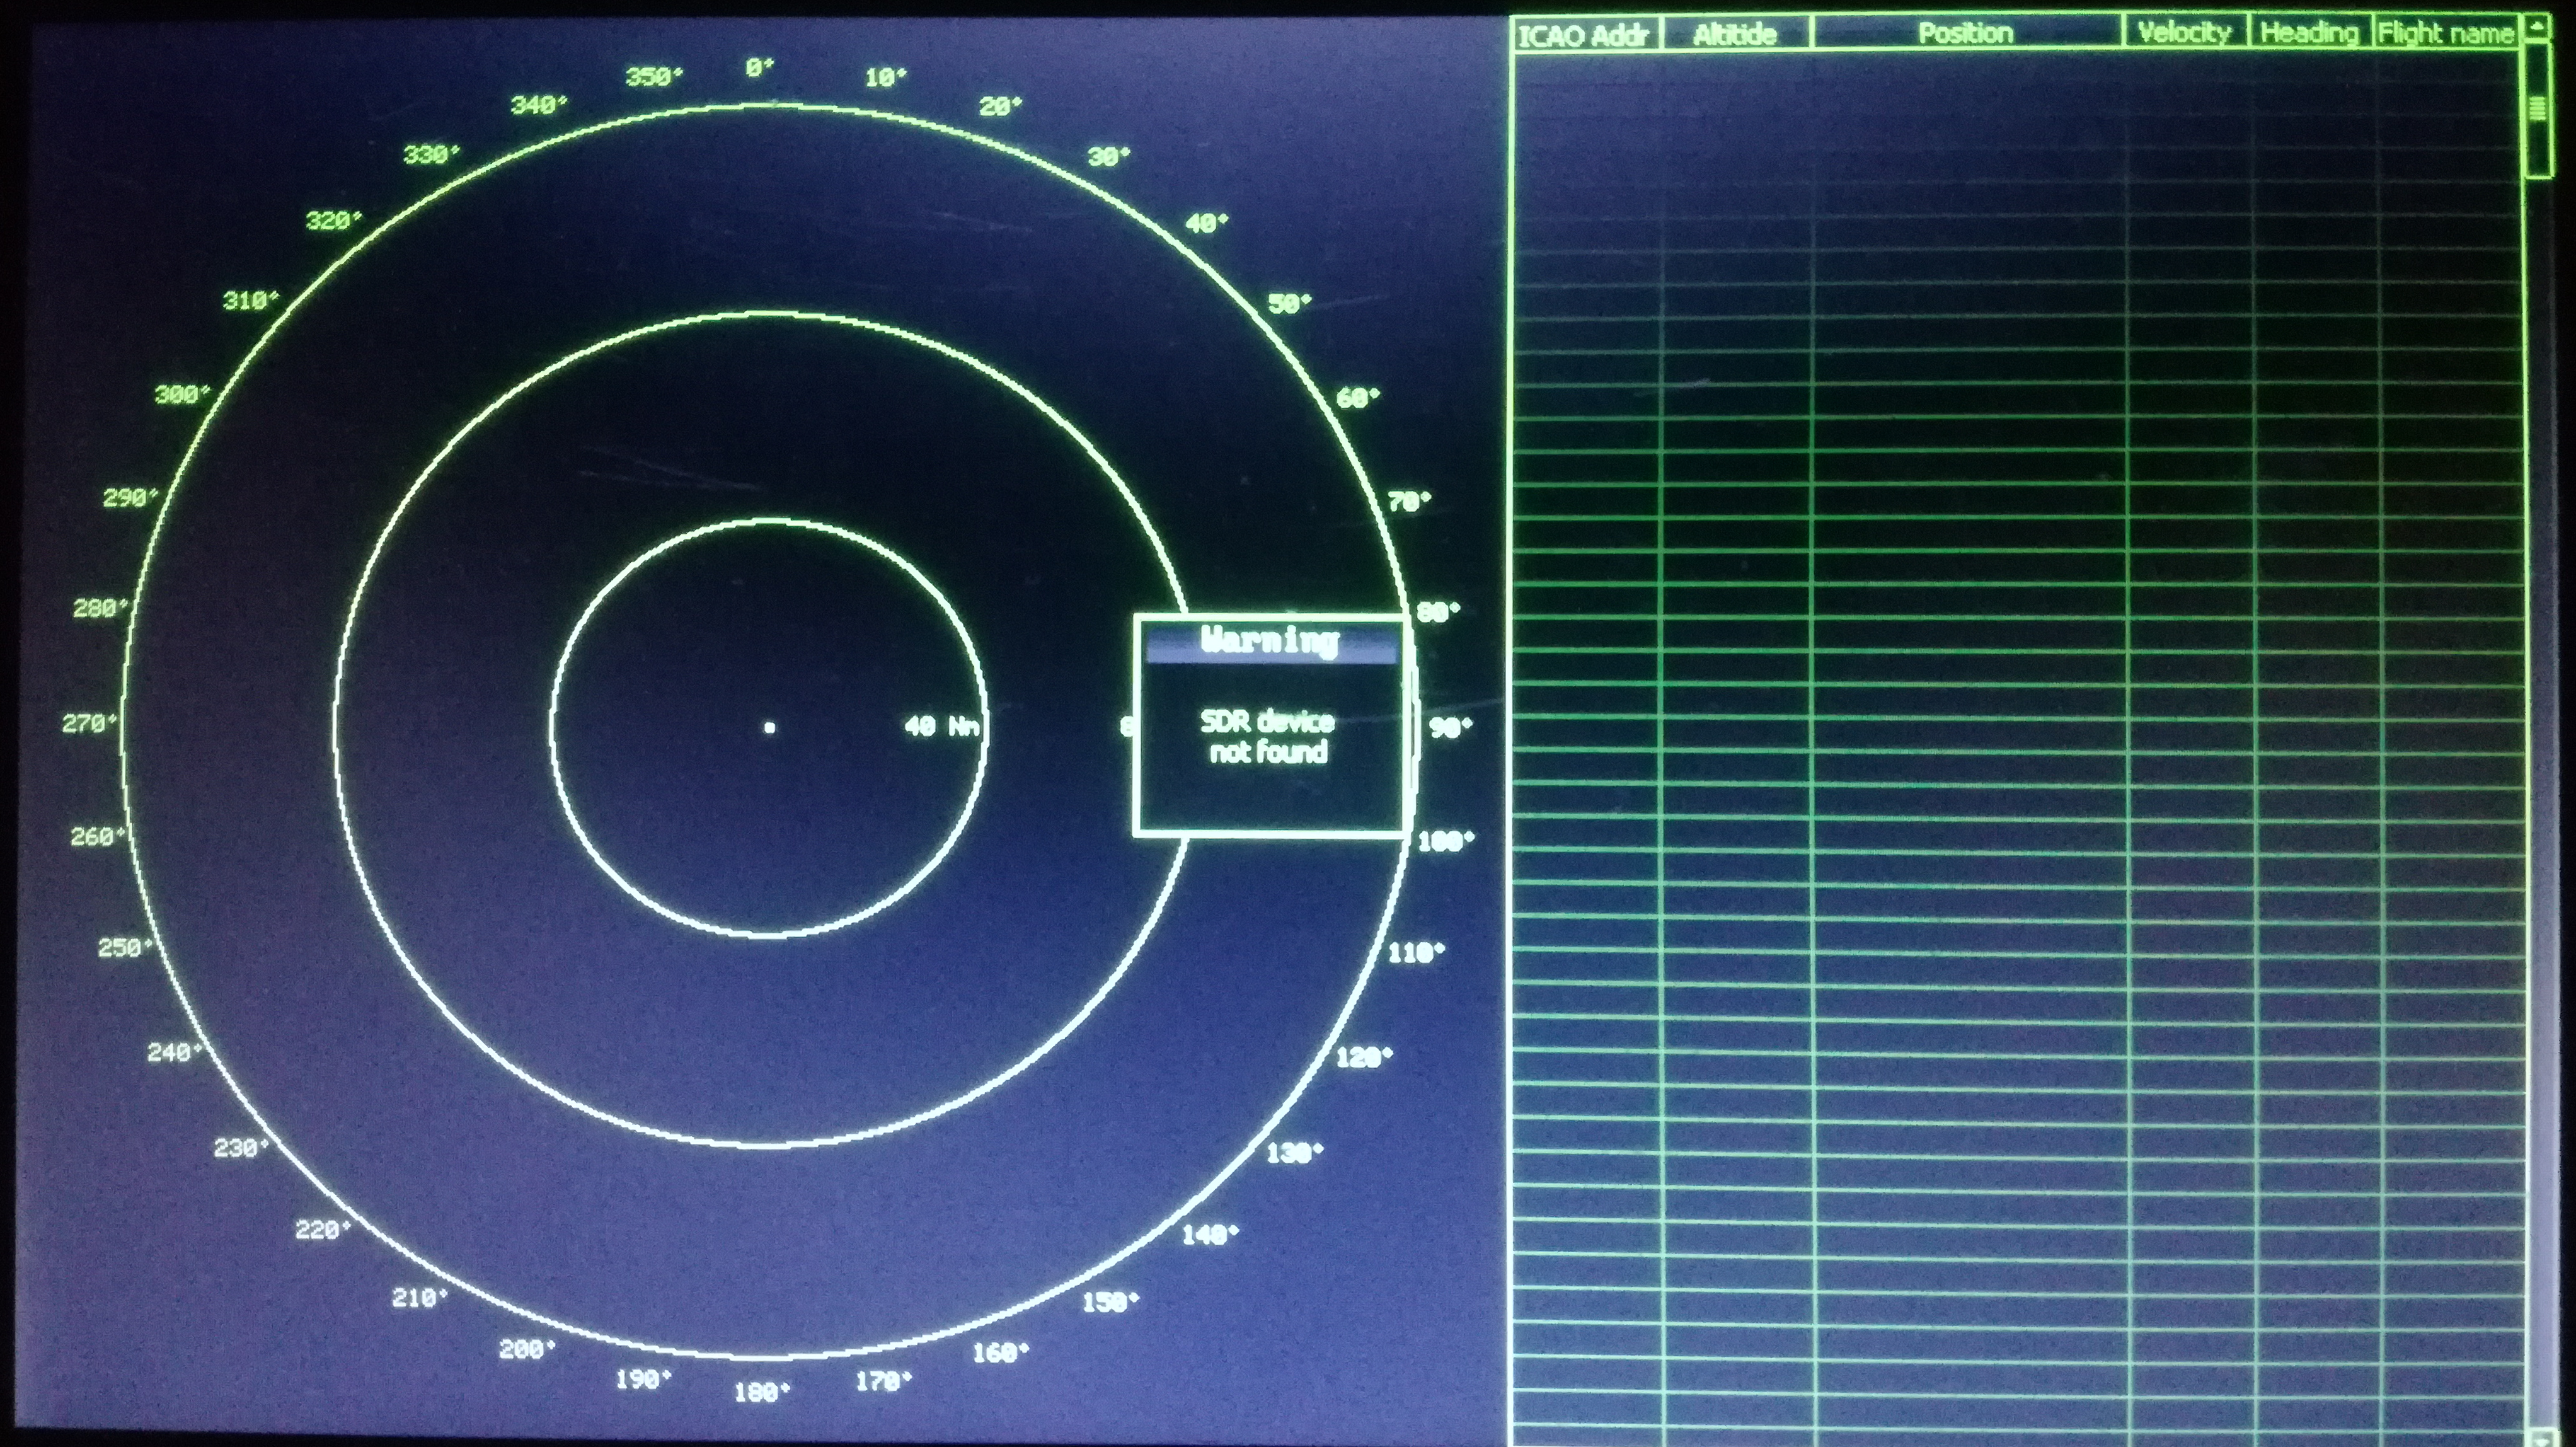
\includegraphics[width=\textwidth]{images/warrning}
    \caption{\textit{Informacja o braku urządzenia SDR}}
\end{figure}
\vskip 1cm
\begin{figure}[!h]
    \centering
    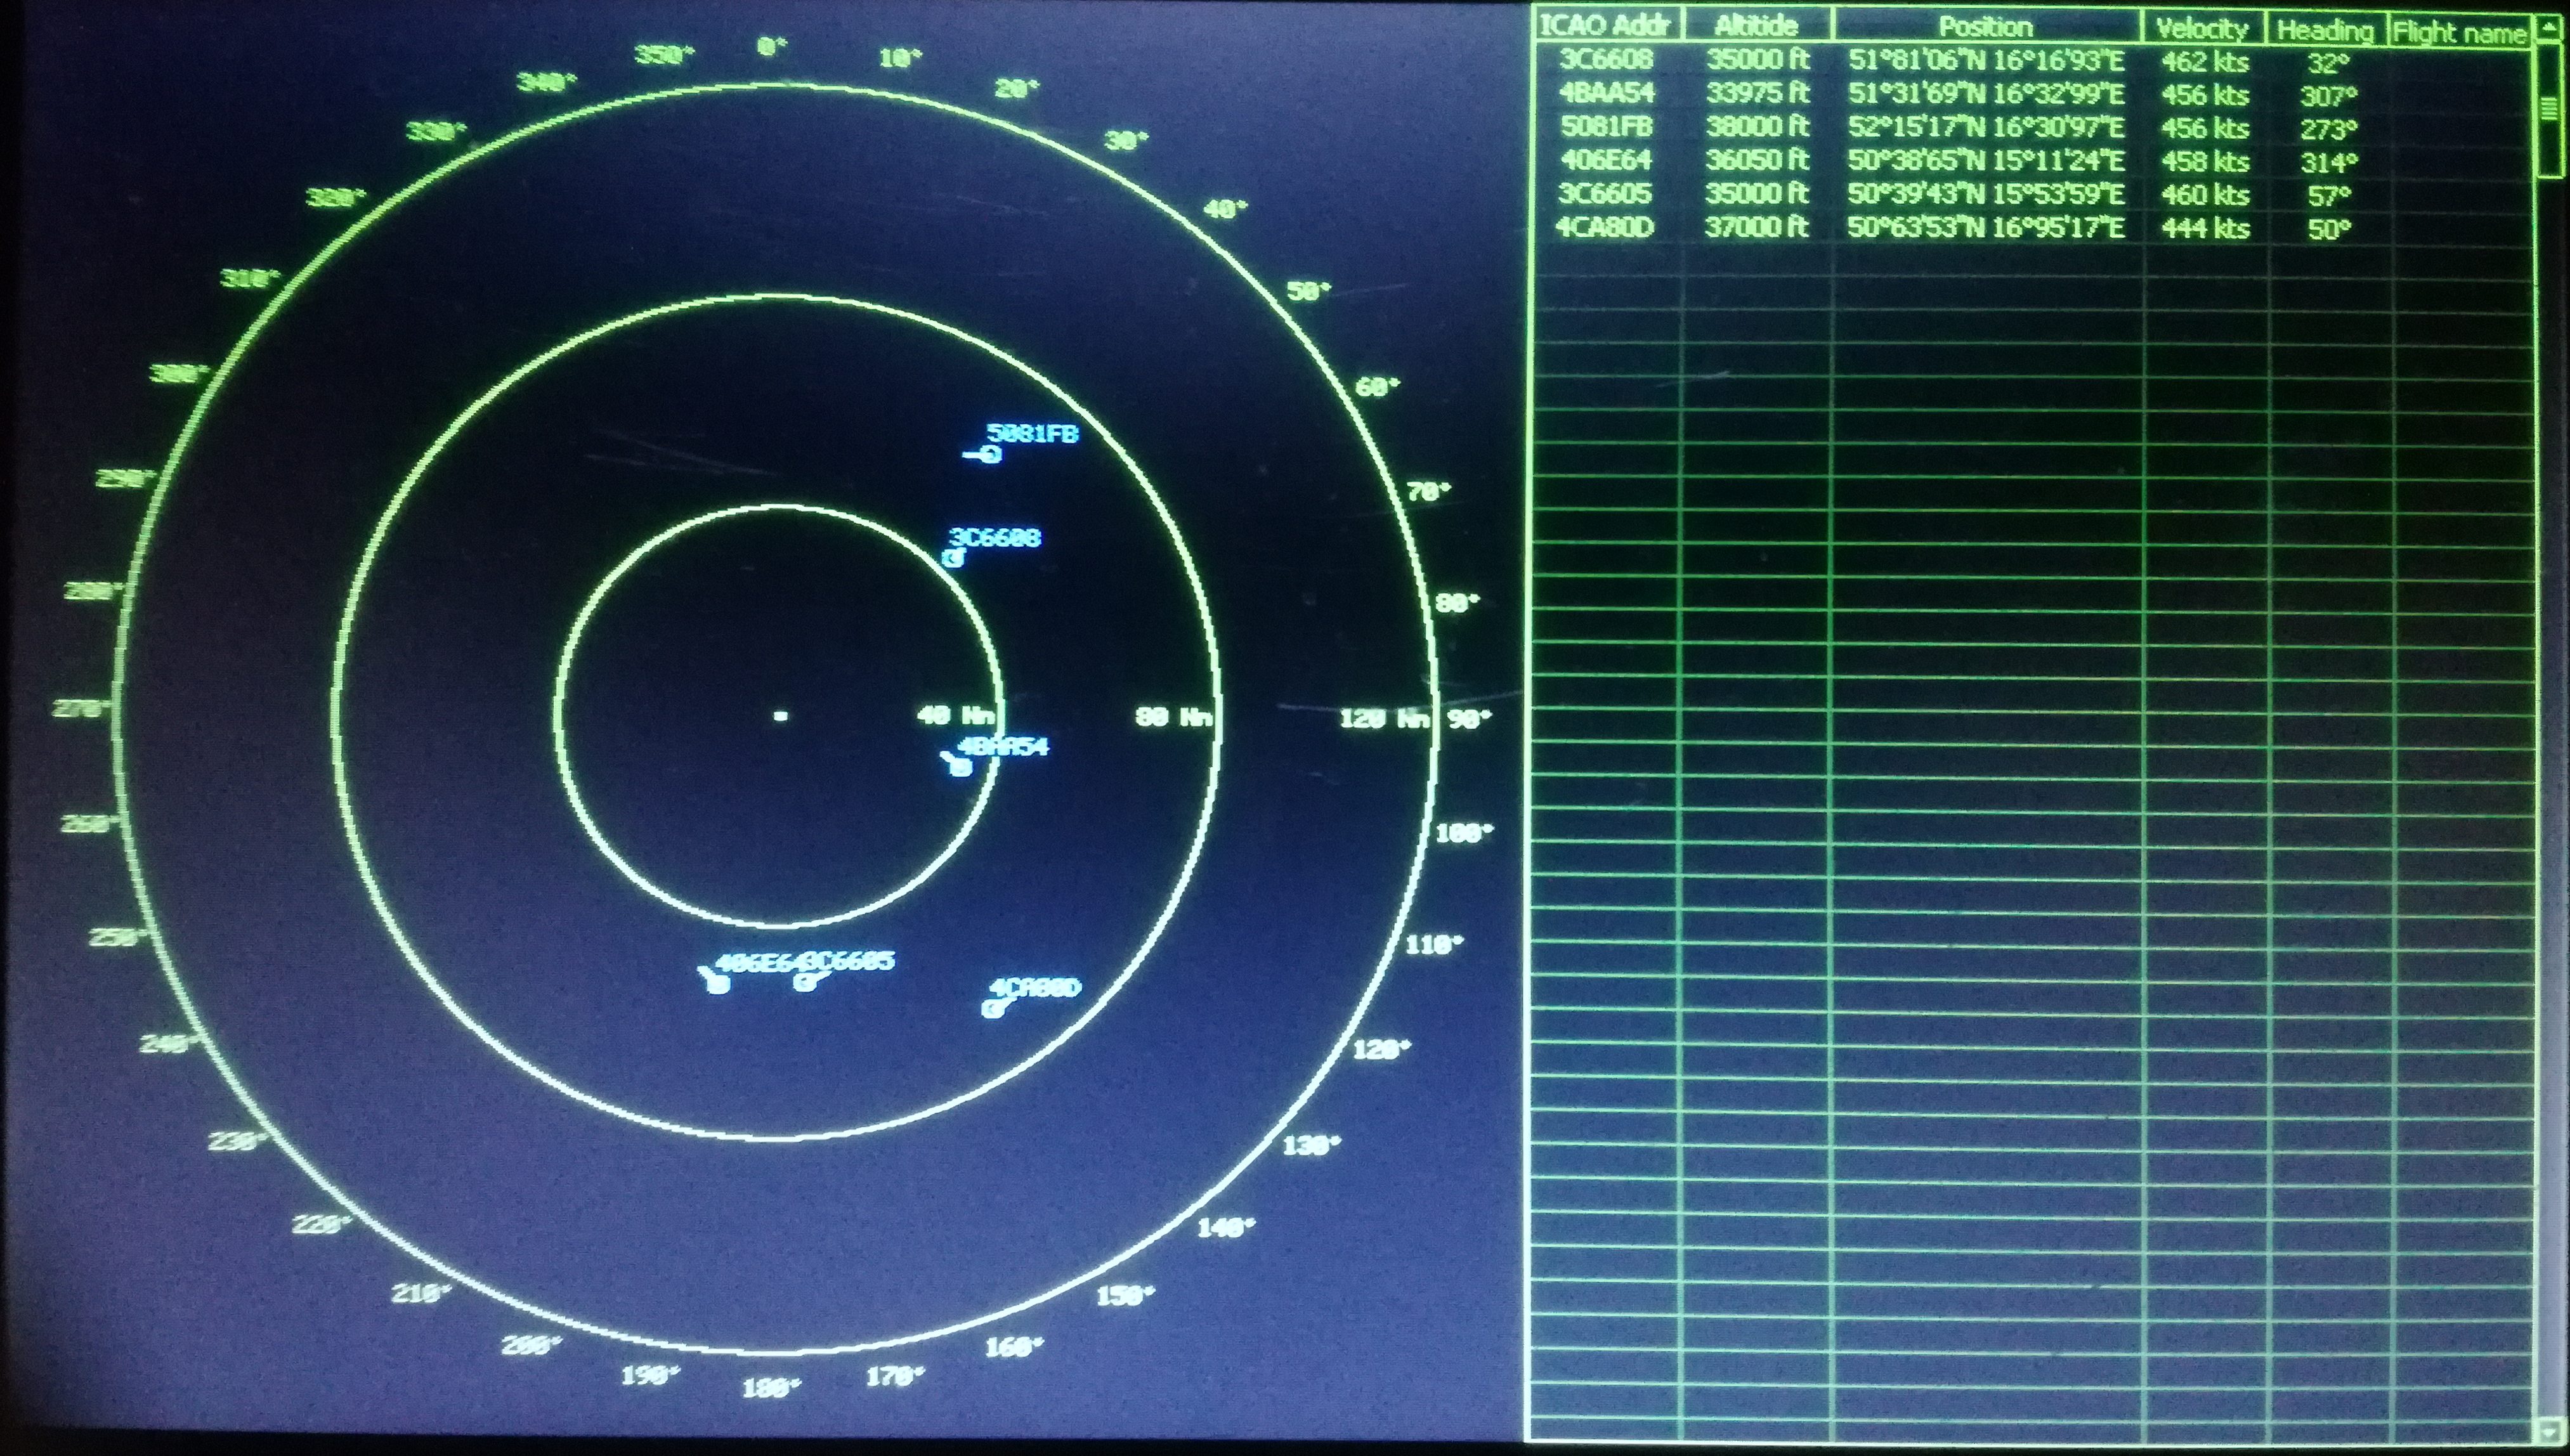
\includegraphics[width=\textwidth]{images/work}
    \caption{\textit{Prezentacja interfejsu użytkownika}}
\end{figure}
\newpage

\chapter{ Podsumowanie }
W tym rozdziale przedstawiano wyniki projektu oraz porównano działanie systemu z innym rozwiązaniem.
\\


Poniżej przedstawiono zdjęcia gotowego urządzenia. Do zasilania wykorzystano akumulator.

\vskip 1cm
\begin{figure}[!h]
    \centering
    \includegraphics[width=\textwidth]{images/deviceTop2}
    \caption{\textit{Zdjęcie gotowego urządzenia}}
\end{figure}
\newpage
\begin{figure}[!h]
    \centering
    \includegraphics[width=\textwidth]{images/deviceBottom}
    \caption{\textit{Zdjęcie tyłu urządzenia}}
\end{figure}

Na rysunku (\ref{fig:testMap}) zaprezentowano porównanie danych ze strony $www.flightradar24.com$ i prezentowanych przez system.

\begin{figure}[!h]
    \centering
    \includegraphics[width=\textwidth]{images/radarTest2.png}
    \caption{\textit{Porównanie pozycji samolotów na radarze i mapie}}
    \label{fig:testMap}
\end{figure}
\newpage
\begin{figure}[!h]
    \centering
    \includegraphics[width=14.5cm]{images/dataTest.png}
    \caption{\textit{Porównanie danych zdekodowanych przez urządzenie i ze strony WWW}}
\end{figure}

Można zauważyć, że pozycja na mapie i radarze nieznacznie się różni. Wynika to z formy prezentowanych informacji. Strona wykorzystuje odwzorowanie walcowe równokątne jako sposób przedstawiania globu w postaci płaszczyzny. Radar pokazuje pozycje statku we współrzędnych biegunowych (kąt i odległość). Zdekodowane dane są poprawne i zgadzają się z prezentowanymi na stronie. Występują niewielkie różnice pomiędzy wyznaczonym położeniem, które wynikają z niedokładności interpolacji położenia samolotu pomiędzy kolejnymi wiadomościami. Urządzenie nie wykryło wszystkich statków powietrznych pokazanych na stronie. Przyczyniła się do tego niewielka antena, która dodatkowo jest uniwersalna, a nie zaprojektowana specjalnie dla częstotliwości 1090MHz. Ponadto system \textit{flightradar24} dysponuje większą liczbą odbiorników.
\\


Wykonane PCB działało poprawnie z wszystkimi komponentami systemu. Udało się nawiązać komunikacje z tunerem DVB-T poprzez interfejs USB, a następnie wykryć i zdekodować przychodzące wiadomości ADS-B. Poprawność zdekodowanych informacji potwierdzono w innym źródle. GUI poprawnie zaprezentowało wpisy z listy.

\addcontentsline{toc}{chapter}{Bibliografia} %utworzenie w spisie treści pozycji Bibliografia
\bibliography{bibliografia} % wstawia bibliografię korzystając z pliku bibliografia.bib - dotyczy BibTeXa, jeżeli nie korzystamy z BibTeXa należy użyć otoczenia thebibliography

\begin{thebibliography}{9}
\bibitem{highSpeedDesign} 
Stephen H. Hal, Garrett W. Hall, and James A. McCall. 
\textit{High-Speed Digital System Design - A Handbook of Interconnects Theory and Design Practices}.
New York, Chichester, Weinheim, Brisbane, Singapore, Toronto, 2000.

\bibitem{digit} 
Richard G. Lyons
\textit{Understanding Digital Signal Processing}.
Eight Printing, 2001.

\bibitem{c++} 
Scott Meyers
\textit{Effective Modern C++}.
Sebastopol, 2014.
 
 \bibitem{c99} 
Brian W. Kernighan, Dennis M. Ritchie
\textit{The C Programming Language}.
New Jersey, 1988.

\bibitem{usbSpec}
Compaq,
Hewlett-Packard,
Intel,
Lucent,
Microsoft,
NEC,
Philips
\textit{Universal Serial Bus Specification}.
Revision 2.0,
2000

\bibitem{usbLayout}
Texas Instruments \textit{High-Speed Interface Layout Guidelines.} \\
http://www.ti.com/lit/an/spraar7g/spraar7g.pdf

\bibitem{frSpec}
\textit{FR408 High Performance Laminate and Prepreg Datasheet.}\\
http://docs.oshpark.com/resources/FR408-High-Performance-Laminate-and-Prepreg-Data-Sheet.pdf

\bibitem{gpsHW}
\textit{LEA-6 / NEO-6 / MAX-6 Hardware Integration Manual.}\\
https://www.u-blox.com/sites/default/files/products/documents/LEA-NEO-MAX-6_HIM_\%28UBX-14054794%29_1.pdf

\bibitem{stmsManual}
\textit{STM32F76xxx and STM32F77xxx advanced Arm®-based 32-bit MCUs Reference Manual}\\
http://www.st.com/en/microcontrollers/stm32f767zi.html

\bibitem{stmsheet}
\textit{STM32F765xx STM32F767xx STM32F768Ax STM32F769xx Datasheet}\\
http://www.st.com/en/microcontrollers/stm32f767zi.html

\bibitem{LTDC}
\textit{LCD-TFT display controller (LTDC) on STM32 MCUs}\\
http://www.st.com/content/ccc/resource/technical/document/application_note/group0/25/ca/f9/b4/ae/fc/4e/1e/DM00287603/files/DM00287603.pdf/jcr:content/translations/en.DM00287603.pdf

\bibitem{dispTiming}
\textit{THC63LVDM83D
24bit COLOR LVDS TRANSMITTER Datasheet}\\
http://www.thine.co.jp/files/topics/169_ext_12_0.pdf

\bibitem{sdram}
\textit{IS42S16400J, IS45S16400J Datasheet} \\
http://www.issi.com/WW/pdf/42-45S16400J.pdf

\bibitem{disco}
\textit{STM32F746G-DISCO schematics}\\
http://www.st.com/en/evaluation-tools/32f746gdiscovery.html

\bibitem{regulator}
\textit{LM1117 800-mA Low-Dropout Linear Regulator Datasheet}\\
http://www.ti.com/lit/ds/symlink/lm1117.pdf

\bibitem{usbPower}
\textit{STMPS2141, STMPS2151, STMPS2161,
STMPS2171 Enhanced single channel power switches}\\
http://www.st.com/en/switches-and-multiplexers/stmps2141.html

\bibitem{emi}
\textit{ECMF02-4CMX8
Common mode filter with ESD protection for USB 2.0 interface}\\
http://www.st.com/en/emi-filtering-and-signal-conditioning/ecmf02-4cmx8.html

\bibitem{dispDesign} 
\textit{HY LCD Reference Design}\\
http://www.hotmcu.com/101-inch-1024x600-tft-lcd-display-with-capacitive-touch-panel-p-215.html?cPath=6_16


\bibitem{adsbDecoding} 
Junzi Sun. 
\textit{ADS-B Decoding Guide}.\\
https://media.readthedocs.org/pdf/adsb-decode-guide/latest/adsb-decode-guide.pdf

\bibitem{manufacturer}
http://docs.oshpark.com/services/four-layer/

\bibitem{posCalc} 
https://www.movable-type.co.uk/scripts/latlong.html

\end{thebibliography}
%opcjonalnie może się tu pojawić spis rysunków i tabel
% \listoffigures
% \listoftables
\end{document}
